\documentclass[fleqn,11pt]{report}

\usepackage[utf8]{inputenc}
\usepackage{textcomp}
\usepackage{booktabs}
\usepackage{amsmath}
\usepackage{natbib}
\usepackage{amssymb}
\usepackage{listings}
\usepackage{color}
\usepackage[svgnames]{xcolor}
\usepackage{graphicx}
\usepackage{endnotes}
\usepackage{sectsty}
\usepackage[a4paper, margin=1.4in]{geometry}
\usepackage[hang,flushmargin]{footmisc}
\usepackage[font=small,labelfont=bf]{caption}
\usepackage[sfdefault,lf]{carlito}
\usepackage[scaled=0.8]{noto}
\usepackage[T1]{fontenc}
%\usepackage{changepage} % adjustwidth
\usepackage{hyperref}
\usepackage{hypcap}
\usepackage{scrextend} % addmargin

\urlstyle{sf}
\widowpenalties 2 10000 0
\clubpenalties 2 10000 0

\sectionfont{\large}
\chaptertitlefont{\LARGE}
\setcounter{secnumdepth}{0}
\definecolor{gray}{rgb}{0.4,0.4,0.4}
\definecolor{darkblue}{rgb}{0.0,0.0,0.6}
\definecolor{cyan}{rgb}{0.0,0.6,0.6}

\lstloadlanguages{C}
\lstset{
  basicstyle=\ttfamily,
  columns=fullflexible,
  showstringspaces=false,
  commentstyle=\color{gray}\upshape
}
\lstdefinelanguage{csharp}{
  basicstyle=\ttfamily\footnotesize,
  morecomment=[l]{//}, %use comment-line-style!
  morecomment=[s]{/*}{*/}, %for multiline comments
  morestring=[b]",
  commentstyle=\color{DarkOliveGreen},
  stringstyle=\color{SaddleBrown},
  identifierstyle=\color{black},
  keywords=[1]{static,class,private,delegate,void,int,public,get,var},
  keywordstyle=[1]\color{DarkBlue},
  keywords=[2]{Func,YCombinator,Program,RecursiveFunc,Console},
  keywordstyle=[2]\color{violet}
}
\lstdefinelanguage{ocaml}{
  basicstyle=\ttfamily\footnotesize,
  morecomment=[s]{/*}{*/},
  morecomment=[s]{(*}{*)},
  identifierstyle=\color{black},
  keywords=[1]{module,type,sig,int,val,let,end},
  keywordstyle=[1]\color{DarkBlue},
  keywords=[2]{MySig,MyModule},
  keywordstyle=[2]\color{violet}
}
\lstdefinelanguage{ts}{
  basicstyle=\ttfamily\footnotesize,
  morecomment=[l]{//}, %use comment-line-style!
  morecomment=[s]{/*}{*/}, %for multiline comments
  morestring=[b]',
  morestring=[b]`,
  morestring=[b]",
  commentstyle=\color{DarkOliveGreen},
  stringstyle=\color{SaddleBrown},
  identifierstyle=\color{black},
  keywords=[1]{function,any,string,if,return,null,undefined,const,interface,extends,type,let},
  keywordstyle=[1]\color{DarkBlue},
  keywords=[2]{getValueByPath,createElement,Document,Node,GlobalEventHandlers,
    NodeSelector,DocumentEvent,ParentNode,TailwindTextColor,Colors,Shades,
    HTMLAnchorElement,HTMLAppletElement,HTMLAreaElement,HTMLAudioElement,HTMLBaseElement,
    HTMLBaseFontElement,HTMLQuoteElement,HTMLBodyElement,HTMLVideoElement,HTMLPreElement,
    HTMLElement,MSHTMLWebViewElement},
  keywordstyle=[2]\color{violet}
}
\lstdefinelanguage{csxml}{
  basicstyle=\ttfamily\footnotesize,
  morestring=[b]",
  moredelim=[s][\color{DarkBlue}]{<}{\ },
  moredelim=[s][\color{DarkBlue}]{</}{>},
  moredelim=[l][\color{DarkBlue}]{/>},
  moredelim=[l][\color{DarkBlue}]{>},
  morecomment=[s]{<?}{?>},
  morecomment=[s]{<!--}{-->},
  commentstyle=\color{DarkOliveGreen},
  stringstyle=\color{SaddleBrown},
  identifierstyle=\color{violet}
}

\begin{document}
\title{\Huge \textbf{Critical Reading of Software}\\~\\}
\author{Tomas Petricek}
\maketitle

% THINGS TO FIGURE OUT:
%
% * is there just too many random architectural references here?
%   (perhaps, but that's what I can do based on my reading...)
% * now its organized by architectural ideas with software scattered around
%   (alternative would be to start from SW - e.g. chapter on TS)
%   (or, at least add SW-centric appendix or interleave?)
%
%


\chapter{Introduction}

The name of the architect Christopher Alexander is perhaps better known in programming
circles than among architects, so he makes for the perfect opening of a text that aims
to find new links between the world of architecture and the world of software. But let
me be clear that I reference Alexander mainly to highlight a question that he posed about
the software practice, rather than to draw inspiration for better software design from his
work, a task already done by others.\endnote{patterns, RPG, Steenson}

The question I want to refer to was raied by Alexander in a keynote that he delivered in
1996 at the annual ACM Conference on Object-Oriented Programs, Systems, Languages and
Applications (OOPSLA). This was not an incidental invitation. By the mid-1990s, Alexander's ideas
on pattern languages and design patterns were already influential in the computer science and
software engineering circles and many of those involved in bringing Alexander's ideas into the
world of software were regular participants at OOPSLA.

In his keynote, Alexander talked about his lifelong quest for creating living structures
in the world, i.e., beautiful structures where each element is in harmony with each other,
structures that evolve well and reflect natural inclinations of their human inhabitants.
In the last part of his talk, Alexander called upon the attendees to take responsibility
for the built environment and tackle the problem of generating living structures.
As Alexander pointed out, the idea of generative process is natural to computer scientists
and so they are well equipped for the task.

Alexander commented on a perceived ``undercurrent of unease as to where all
this---software design---is going''. In a ``very direct and blunt'' comment, he suggests that:

\begin{quote}
It could be thought that the technical way in which you [computer scientists] currently look at
programming is almost as if you were willing to be ``guns for hire.'' In other words, you are the
technicians. You know how to make the programs work. ``Tell us what to do daddy, and we'll do it.''
That is the worm in the apple.
\end{quote}
% https://www.patternlanguage.com/archive/ieee.html

One could conclude that computer scientists and programmers share their predicament with architects
who, as argued by Charles Jencks\endnote{p26} ``have little power, [and] are not in any better
position to command what is built.'' Perhaps like architects, computer scientists and programmers
being ``fairly low in the chain of command and needing jobs, are prone to compromise with the
state and the establishment.''

There may be some truth in that, but I believe this is not the entire truth. On a more basic level,
programming, computer science and software development lack the critical language that is needed
for thinking about the problem. In other words, regardless of whether we have the power to command
what is built, we do not know how to effectively critically question what is built, how to imagine
alternatives, and how to ironically poke at the undesirable characteristics of what is being built.

\section{Critical Language for Software}
This text is an attempt to develop such critical language of software. To do so, I will draw on
a number of architects and architectural critics. Their work provides an inspiration for
what, I believe, is needed for software. Some of those critiques are in the form of written text,
but more notably, architects also use building plans and buildings themselves to raise important
points about architecture. I believe we, programmers and computer scientists, similarly need to
find ways of designing software that not only fulfils a certain function, but also raises critical
questions. I acknowledge a certain irony in my effort. What you are looking at is itself text
and not a piece of software.

Although I started with Alexander's comment and I share his belief that programmers and computer
scientists should not accept the role of ``guns for hire,'' my thinking follows a different
route than that suggested by Alexander---one that would likely not make Christopher Alexander
himself very happy.\endnote{Alexander Eisenmann debate \url{https://arahovsepyan.com/eisenmanalexander}}
Rather than seeking a way of building that achieves a living structure, I turn to debates
on architecture that emerged from post-modern critical architecture and debates about it.

Even if our sole goal as programmers and computer scientists was to produce ``living
structures'' in the world, I do not think we can achieve this without first having a critical
language that lets us reflect on our work, criticise existing approaches, deconstruct our creations
and look for alternative arrangements.

In other words, I believe there is a value in exploring disharmony\endnote{Agreeing with Eisenmann
in the debate} and in using a critical language of architecture---or in my case of software---to
criticise the state of the discipline and imagine new ways of thinking and new ways in which
software can support social structures. Although I mainly look to writing on post-modern ar
chitecture for sources of inspiration, the idea of using buildings to question established order
is by no means new. We can trace similar ideas to the rise of modernism in Europe following
the First World War when some architects ``overwhelemed by the nightmare of industrialization
(...) briefly speculate on alternative condition'':\endnote{Oppositions -- p52, p55}

\begin{quote}
It is not the crazy caprice of a poet that glass architecture will bring a new culture.
It is a fact. (\ldots) Therefore the European is right when he fears that glass architecture
might become uncomfortable. Certainly it will be so. And that is not its least advantage.
For first of all the European must be wrenched out of his coziness.
\end{quote}

On the next couple of pages, I will look at two themes from post-modern architecture that
highlight some of the aspects of the critical language developed by architects that I hope
to create for software. I will then return to methodological problem of how such language
can be structured.

\newpage

\begin{figure}
\includegraphics[height=9.85em]{chapters/fig/columns-archives.jpg}\quad
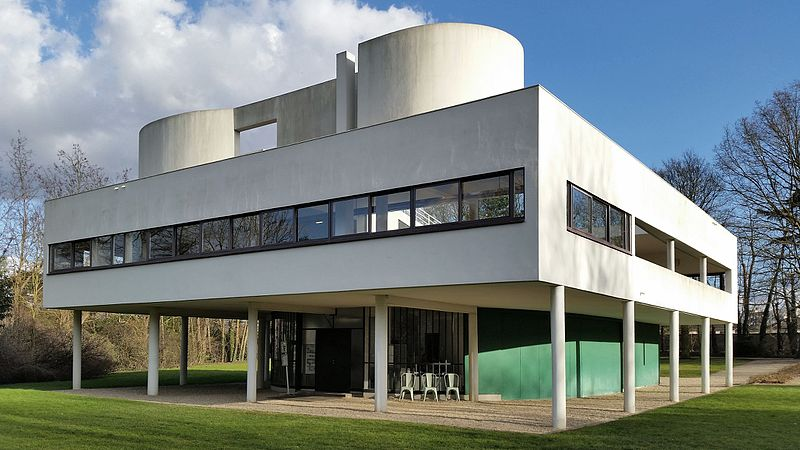
\includegraphics[height=9.85em]{chapters/fig/columns-savoye.jpg}\quad\\[1em]
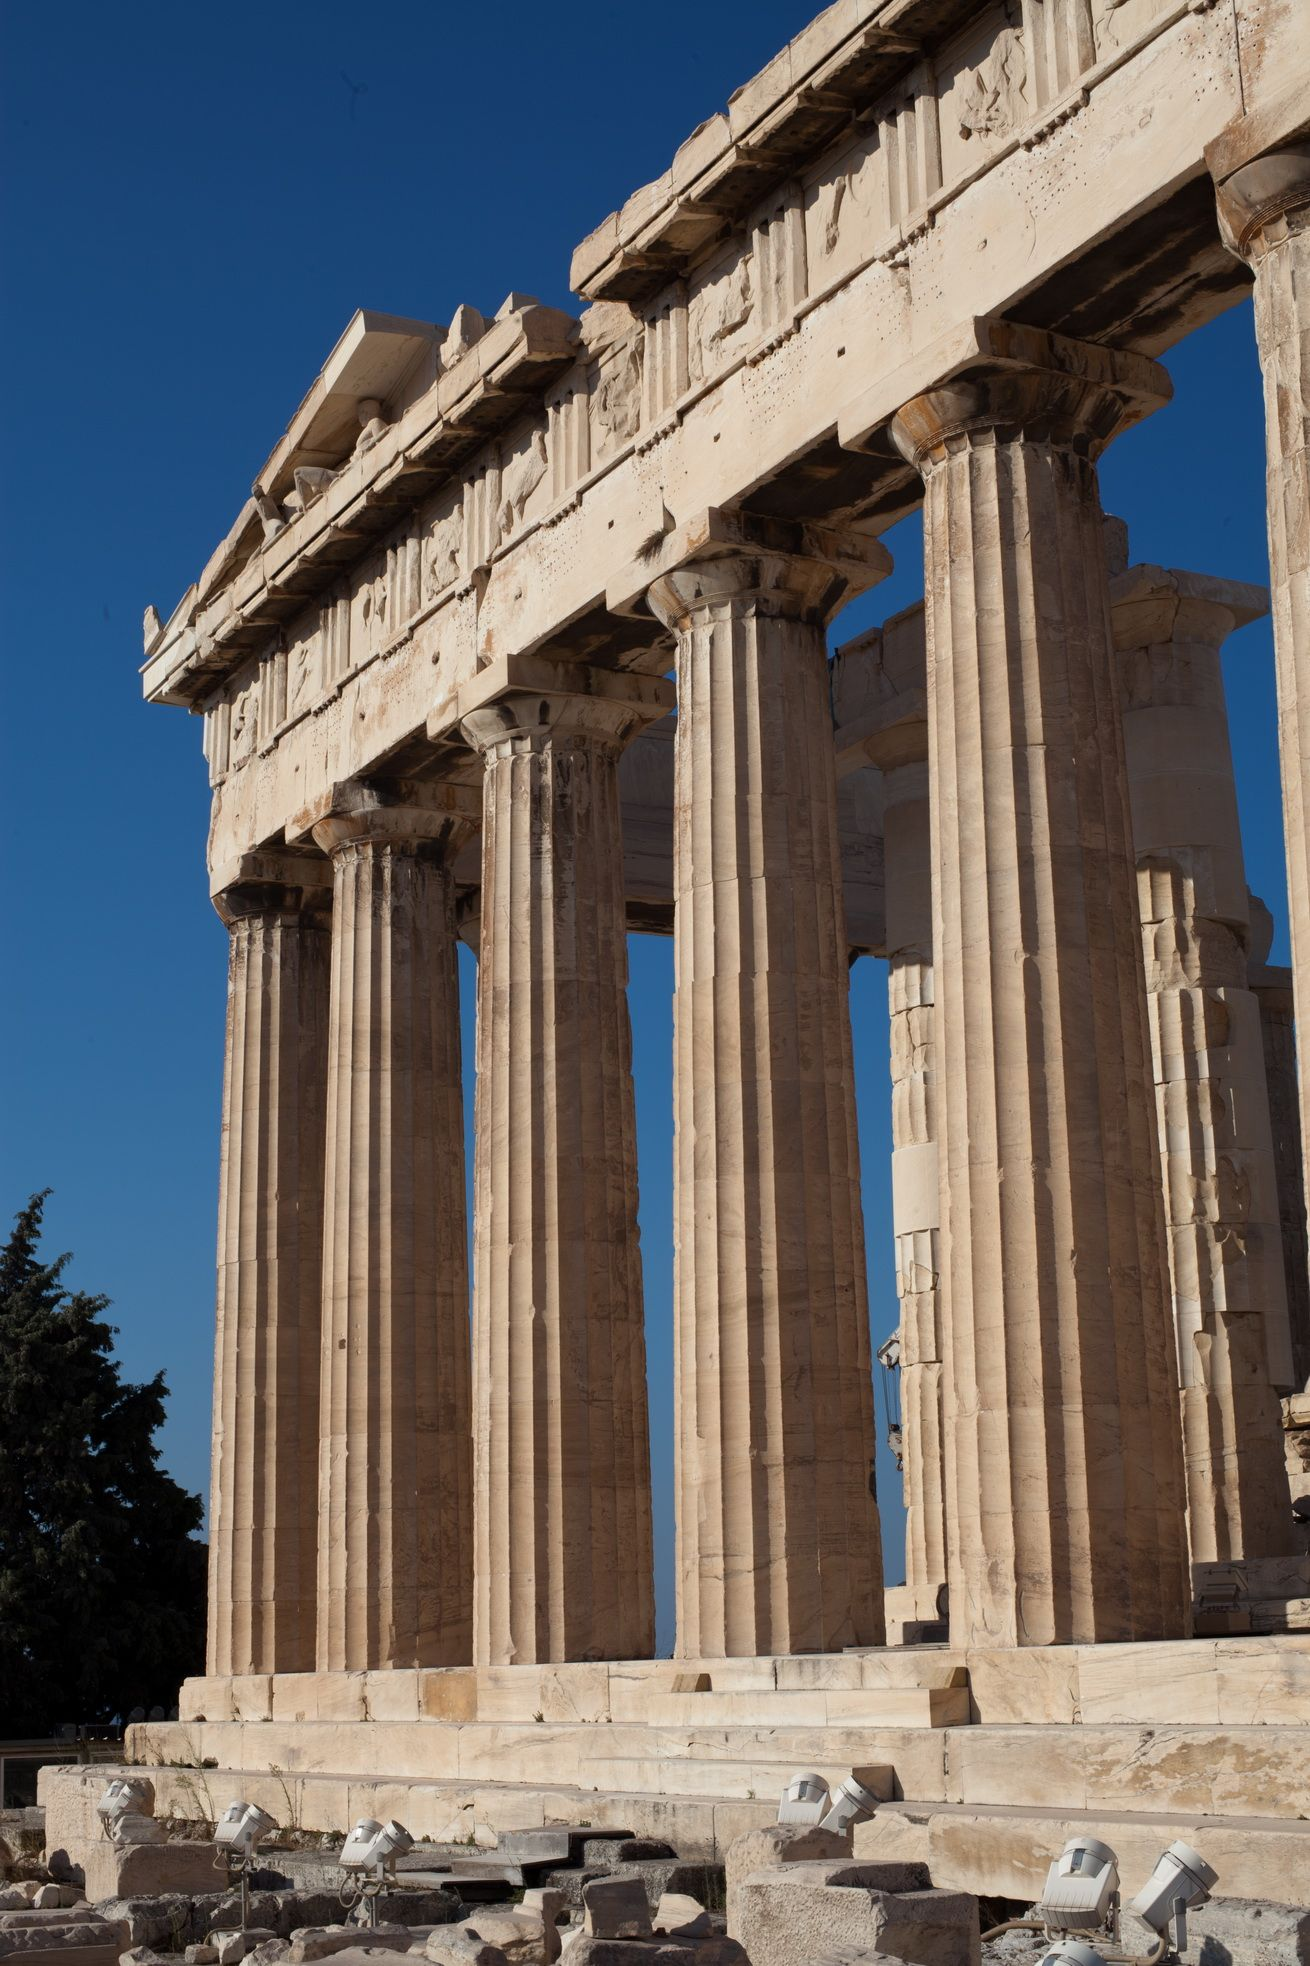
\includegraphics[height=12em]{chapters/fig/columns-greek.jpg}\quad
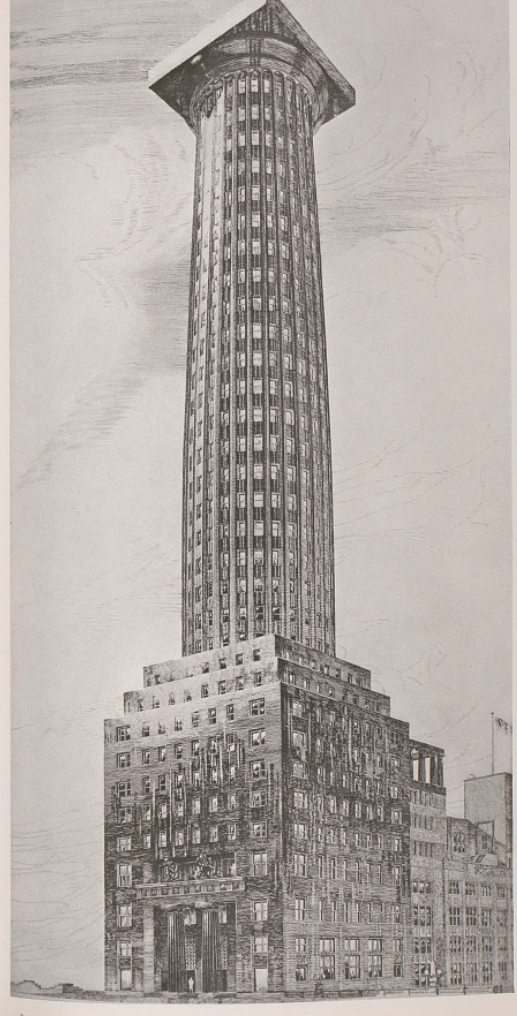
\includegraphics[height=12em]{chapters/fig/columns-loos.png}\quad
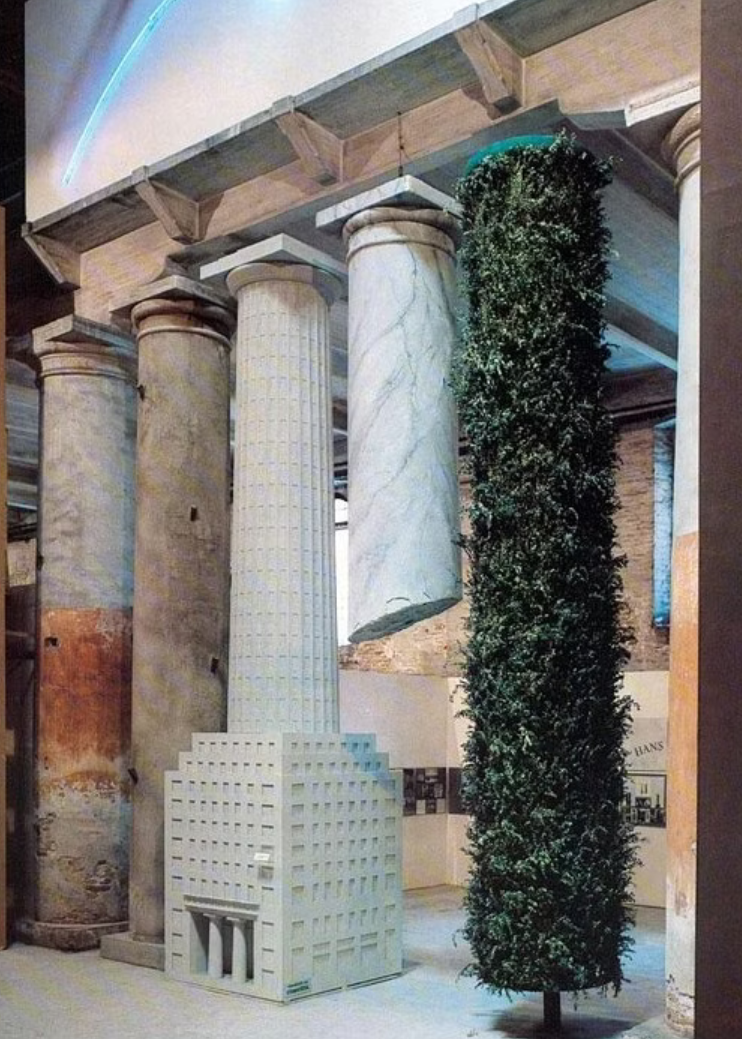
\includegraphics[height=12em]{chapters/fig/columns-venice.png}\quad
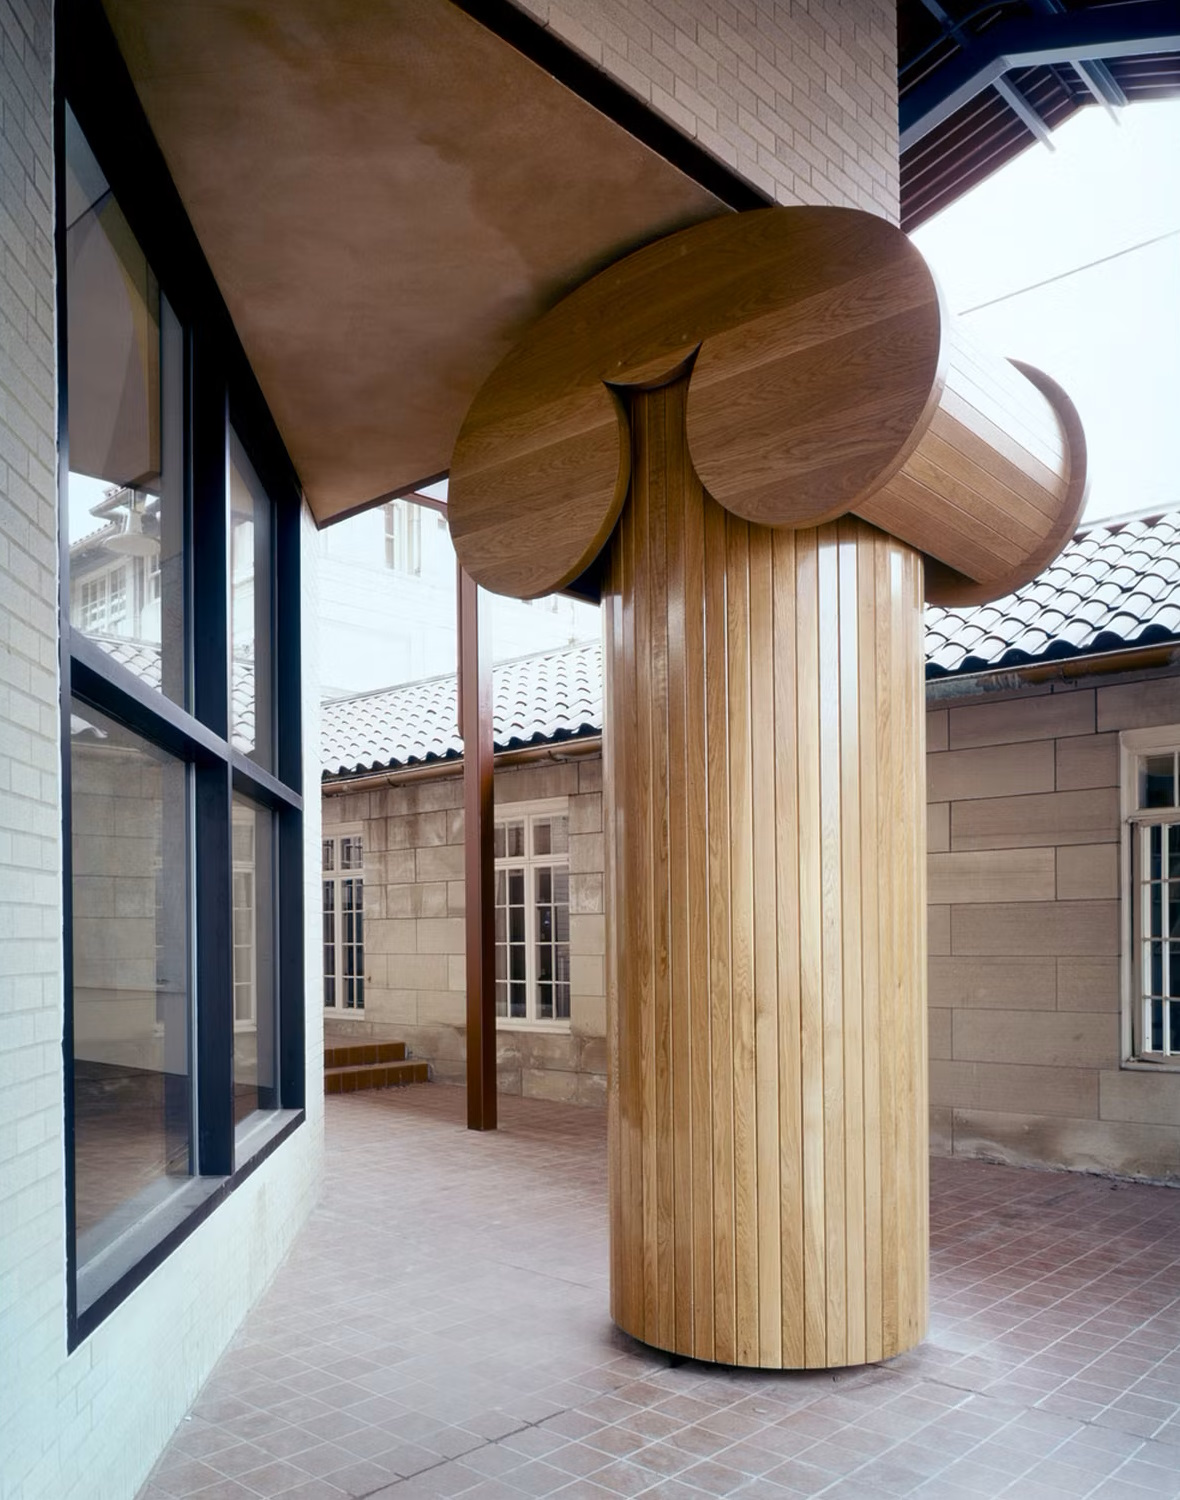
\includegraphics[height=12em]{chapters/fig/columns-venturi.jpg}
\caption{Six different uses of columns in architecture. (1) Unironical use of the column in the 1935
neoclassical building of the US National Archives, (2) Supporting pilotis in Le Corbusiers 1931
Villa Savoye, (3) The Parthenon in Athens built in the 5th century BC according to the Doric order
(4) Adolf Loos' playful reference to the Doric column in a 1922 entry for the Chicago Tribune
Tower Competition, (5) Hans Hollein's ironical Facade of Morphed Columns, at the 1980 Venice
Architecture Biennale, and (6) Robert Venturi's ``ironic'' column from the 1977 addition to the
Allen Memorial Art Museum.}
\label{fig:columns}
\end{figure}

\section{The Ironical Column}
To illustrate some of the ways through which architects use architecture to communicate, I start
with the most basic structural element of classical architecture, the column. Figure~\ref{fig:columns}
shows several uses of columns, starting from the ancient Parthenon built in Athens in 5th century
BC (bottom left) followed by four examples that include a variety of references to the classical
column.\endnote{Idea from Oppositions p377, See also Korman ``The Architecture of the Facade'' -
for more on columns}

Neoclassical architecture, which gradually grew in prominence in the late 18th century, looks
back to the Classical past. It sees it as a source of pure geometric order with ideal proportions
and symmetry. Such references to the ancients should not be unexpected. At the start of the 17th
century, Aristotle and other ancient philosophers were seen as the source of truth that was partly
lost and needs to be recovered, but that was already fully known to the ancients.\endnote{Wootton}
The scientific revolution of the 17th century gradually changed perspective on the ancients in what
was becoming experimental science, but it should not be a surpirse that architects of the 18th century
were still looking back to ancient structures that were becoming rediscovered and better understood
at the time. Neoclassical architecture remained influential after the 18th century, but its meaning
slowly shifted. It turned from an attempt to rediscover and recreate simple, purely geometrical
structures to an idealized style that emphasises tradition. The use of the style for many US federal
buildings is thus a reference to the values that the style encompasses.\endnote{Also conservative
``Executive Order on Promoting Beautiful Federal Civic Architecture'' -- Trump's administration (2020)}

The modernist Villa Savoye designed by Le Corbusier also looks back to the Classical past,
but it does so in a different way. Rather than directly copying the style and order of the
ancient Greek temples, the building is a reinterpretation of the ideas of a Greek
temple.\endnote{Unwin - Twenty-Five Buildings Every Architect Should Understand}
It reimagines the ideal structure of Greek temple based on geometric principles (using the golden
ratio), but replaces ancient Greek columns with minimalistic modernist pilotis. Following the
modernist focus on function, Le Corbusier's design uses pilotis to give prominence to the
automobile (parked on the ground floor). Although the same historical reference is present in Villa
Savoye, it is used at a more conceptual level and is not immediately apparent.

The importance of the column as an icon representing a certain style of architecture was well
understood by other modernist architects, including Adolf Loos who is best known as the author
of the modernist manifesto ``Ornament and Crime'', first presented as a lecture in 1910. In his entry
for the Chicago Tribune headquarters competition in 1922, Loos made yet another reference to the
ancient Greek temple and shaped the entire building as a giant Doric column.  Loos himself did not
view the column in his design as ornamental and instead saw it as supporting the public nature of
the building with appropriate symbolism.\endnote{Krul - Adolf Loos and the Doric Order}
The structure of the building itself here becomes the symbol in a way that is reminiscent
of later post-modernist works where construction patterns and material textures themselves become
ornament.\endnote{Jencks, p183} Despite being rooted in the modernist thinking, the Chicago Tribune
Tower project became an inspiration for later post-modern architects who make, more or less subtle,
historical references in an ironic way. They will include columns in their buildings to indicate
that they recognize being a part of architectural culture and tradition, even if they no longer
need columns as structural support mechanisms.

A good illustration of the ironic reference is the facade created by Hans Hollein for the 1980
Venice Biennale. The event took place in Corderia of the Arsenale, a large historical building
itself featuring supporting columns. The participants of the Biennale were asked to design a
facade for their exhibition that would cover (and hide) the historical structure of the Corderia.
Hollein did the exact opposite. He complemented two columns of the Corderia with a range of
ironical forms of columns. One was a bushy tree cut into the shape of a column, while another was
a scaled-down version of Loos' Chicago Tribune Tower. The entrance into the exhibition was under
a hanging fragment of a column, which clearly lost its original structural function, but gained
a different function as an exhibition entrance. Here, the ironical use of the architectural
language is direct and understandable.\endnote{Branscombe - Hans Hollein and Postmodernism}

Hollein's entry addressed the theme of the Biennale, ``The Presence of the Past'' in a way that
is funny and ironic, but sends a clear message about history and continuity of architecture. It
also illustrates the changing function of a column from supporting structure to a decoration. Moreover,
the ironical style of the presentation, shared with many other post-modern architectural works, makes
the message accessible and engaging for broader public. Hollein's facade is interesting for
yet another reason. It uses architectural language to communicate architectural ideas, but it
is neither text, nor a building. As we will see repeatedly, built structures such as stage sets
or monuments are often interesting media through which critical architectural ideas can be
expressed.

The column takes yet another form in the addition to the Allen Memorial Art Museum designed by
Robert Venturi in 1977. The extension itself is based on an idea that Venturi refers to as
the ``decorated shed''. The basic structure and spatial disposition of the building itself is
simple and serves its function which was, in part, to provide more storage space.
Any symbolic, cultural and aesthetic meaning is provided ``by modifying the basic shell by means
of design decisions of a second order.''\endnote{Oppositions, p182} One such second-order
decision is the addition of isolated iconic elements, such as the mock Ionic column that
marks the building as cultural institution. In a way, the column serves similar role as the
neoclassical architecture of the US National Archives, but is here added merely as an ironic
decoration. The association of ancient Greek columns with important public buildings remains,
but the story is told in a very different way.

% ~
%
% ~
%
% "Classicist tropes estranged from traditional use" - Aureli
%
%
% ironic historical reference - critical of neoclassicism
% change of function, repurpose
% exhibition - stage set / pavilons, allows for communication
% reveal inherent conflicts
% ironically distort regularity - point out things
% change of function - non-structural (decorated shed)
% irony valued for superior depth, allows showing multiple contradictory views (Jencks, 79)
% intellectual reference to other works vs. funny reference for broader public - to engage with wider audience!

\section{Towards Critical Software}

In my attempt to translate the critical langauge of architecture into the world of software,
I will alternate between two modes of working. First, I will reinterpret existing practices
in software development and computer science in light of the architectural theory. Second,
I will suggest how we could more deliberately follow in the footsteps of architects and
create new software artifacts that express critical points about software.

In other words, can we follow post-modern architects and embed criticism as a first-class
element in software practice, rather than leaving it to a second-class (and largely optional)
critical writing?\endnote{Oppositions 377, also Venturi introduction} We can also look to
post-modern architects for initial ideas of what such critical software can say. The
architectural style known as eclecticism makes funny references such as Hans Hollein who
decorated his Austrian Travel Agency office with metalic palm trees and broken Greek
column.\endnote{Jencks, p56} The appeal of the style is not just its straightforward humour,
but the fact that it is understandable and can communicate with wider audience. Similarly,
post-modern architects have used contextualism to highlight important characteristics of the
environment they work in or use references to suggest alternative social organization.

Looking at existing software practices, we can imagine how the above arhictectural ideas
can apply to basic structural elements from which software is built. One such element may
be the data structures around which software is structured.\endnote{ref Abstracting craft p96;
ref Joel - the other part of the basic structure is how change is described} Data structures
in software are arguably even more fundamental than columns in architecture, because any
software that works with data needs to store the data in some way. The limitation of this
metaphor is that, unlike columns which are typically visible, data structures are typically
hidden from the end-user. There also is no singular classical model of data structures,
although a number of models fit a similar role. These include the relational model of databases,
flat memory model of low-level programming languages and data types that model data as collections
of nested records.\endnote{Memory models blog}

We can use the architectural metaphor to talk about the differnt kinds of classical models
of data structures. Whereas the relatively expressive language of the relational model or
the nested records model could be linked to different kinds of classical columns, the minimalistic
models of flat memory or nested lists of the Lisp programming language are more akin to
modernists undecorated and purely functional pilotis.

When the data structures are used to store data, they serve the original intended purpose,
just like columns functioning as supporting structure. But equally, there are software systems
where data structures are used more as rhetorical elements, intended not for the computer
execution of the software, but for the end-user or programmer. One example would be types
in the TypeScript programming language. Here, the actual representation of data can be anything
permitted by the underlying JavaScript runtime. TypeScript type declarations are mere labels,
intended for the human and for the static TypeScript type checker, but they are not enforced or
used for checking at runtime. The type declarations still look like a definition of the shape
of a data structure (a column), but they no longer play the basic structural function. They are
used for paratial checking (a scaffolding around a column?) and as information for the
programmer (a purely rhetorical column). A similar case would be the use of data structures
in non-relational databases such as key-value stores or document databases. The data stored
in such systems in practice has some implicit structure.  However, any explicit description
of the structure is merely literal. The description may use the language of standard data
structures (collections, records, primitive types), but this is not used for representation.

Do certain data structures also have particular symbolic associations, in a manner similar
to how the Classical column stands for traditional values, often associated with US federal
buildings? I believe this is the case. For instance, the class-based object-oriented
programming paradigm is often associated with maintainability. Languages that adopt
class-based object-oriented abstractions as their basic data structure do not do so
just for practical, but also for symbolical reasons. TypeScript serves to illustrate this
again. One of the first books on the language claims that ``TypeScript [brings] a level of
maintainable structure to JavaScript development through its class and module
features.''\endnote{Dan Maharry, TypeScript Revealed, 2013} Written in the same year when
the language was released, the claim could not rely on empirical experience with the language,
but mainly on the symbolic associations of the data structure.

\begin{figure}
\begin{lstlisting}[language=csxml]
<CsamlFile xmlns="http://schemas.microsoft.com/winfx/2006/xaml/csaml"
      xmlns:x="http://schemas.microsoft.com/winfx/2006/xaml">
  <NamespaceDeclaration Identifier="MyNamespace">
    <ClassDeclaration Identifier="MyClass" Access="Public">
      <MethodDeclaration Identifier="Main" Access="Public"
            Modifier="Static" ReturnType="{x:Type void}">
        <InvocationExpression MemberAccess="System.Console.WriteLine">
          <InvocationExpression.ArgumentList>
            <Literal Type="{x:Type string}" Value="Hello, CSAML!">
          </InvocationExpression.ArgumentList>
        </InvocationExpression>
      </MethodDeclaration>
    </ClassDeclaration>
  </NamespaceDeclaration>
</CsamlFile>
\end{lstlisting}
\caption{The ``Hello world'' program written using the C\# Application Markup Language (CSAML),
conceived by Charles Petzold in an April Fool's post on 1 April 2006.}
\label{fig:csaml}
\end{figure}

For my last example based on a reference to an existing artefact, I want to show that
data structures have already been used to make critical ironical statements. The April Fool's
post written by Charles Petzold in 2006 introducing the ``C\# Application Markup Language''
is a illustration.\endnote{\url{http://www.charlespetzold.com/etc/CSAML.html}}
The post introduces a new notation that encodes programs written in the C\# language
using XML (Figure~\ref{fig:csaml}). The post can be seen as an ironical work of contextualism.
The post was published in the heyday of the XML format when Microsoft released multiple
development frameworks built around XML. As a well-written April Fool's joke, the post
made readers think. The post praises the semantic clarity of the XML format and gives
various examples that are extremely lengthy and tedious. After a brief puzzlement, most readers
realise the joke. But the post makes them wonder about the verbosity and unnecessary
overuse of the format at the time.

\begin{figure}
\centering
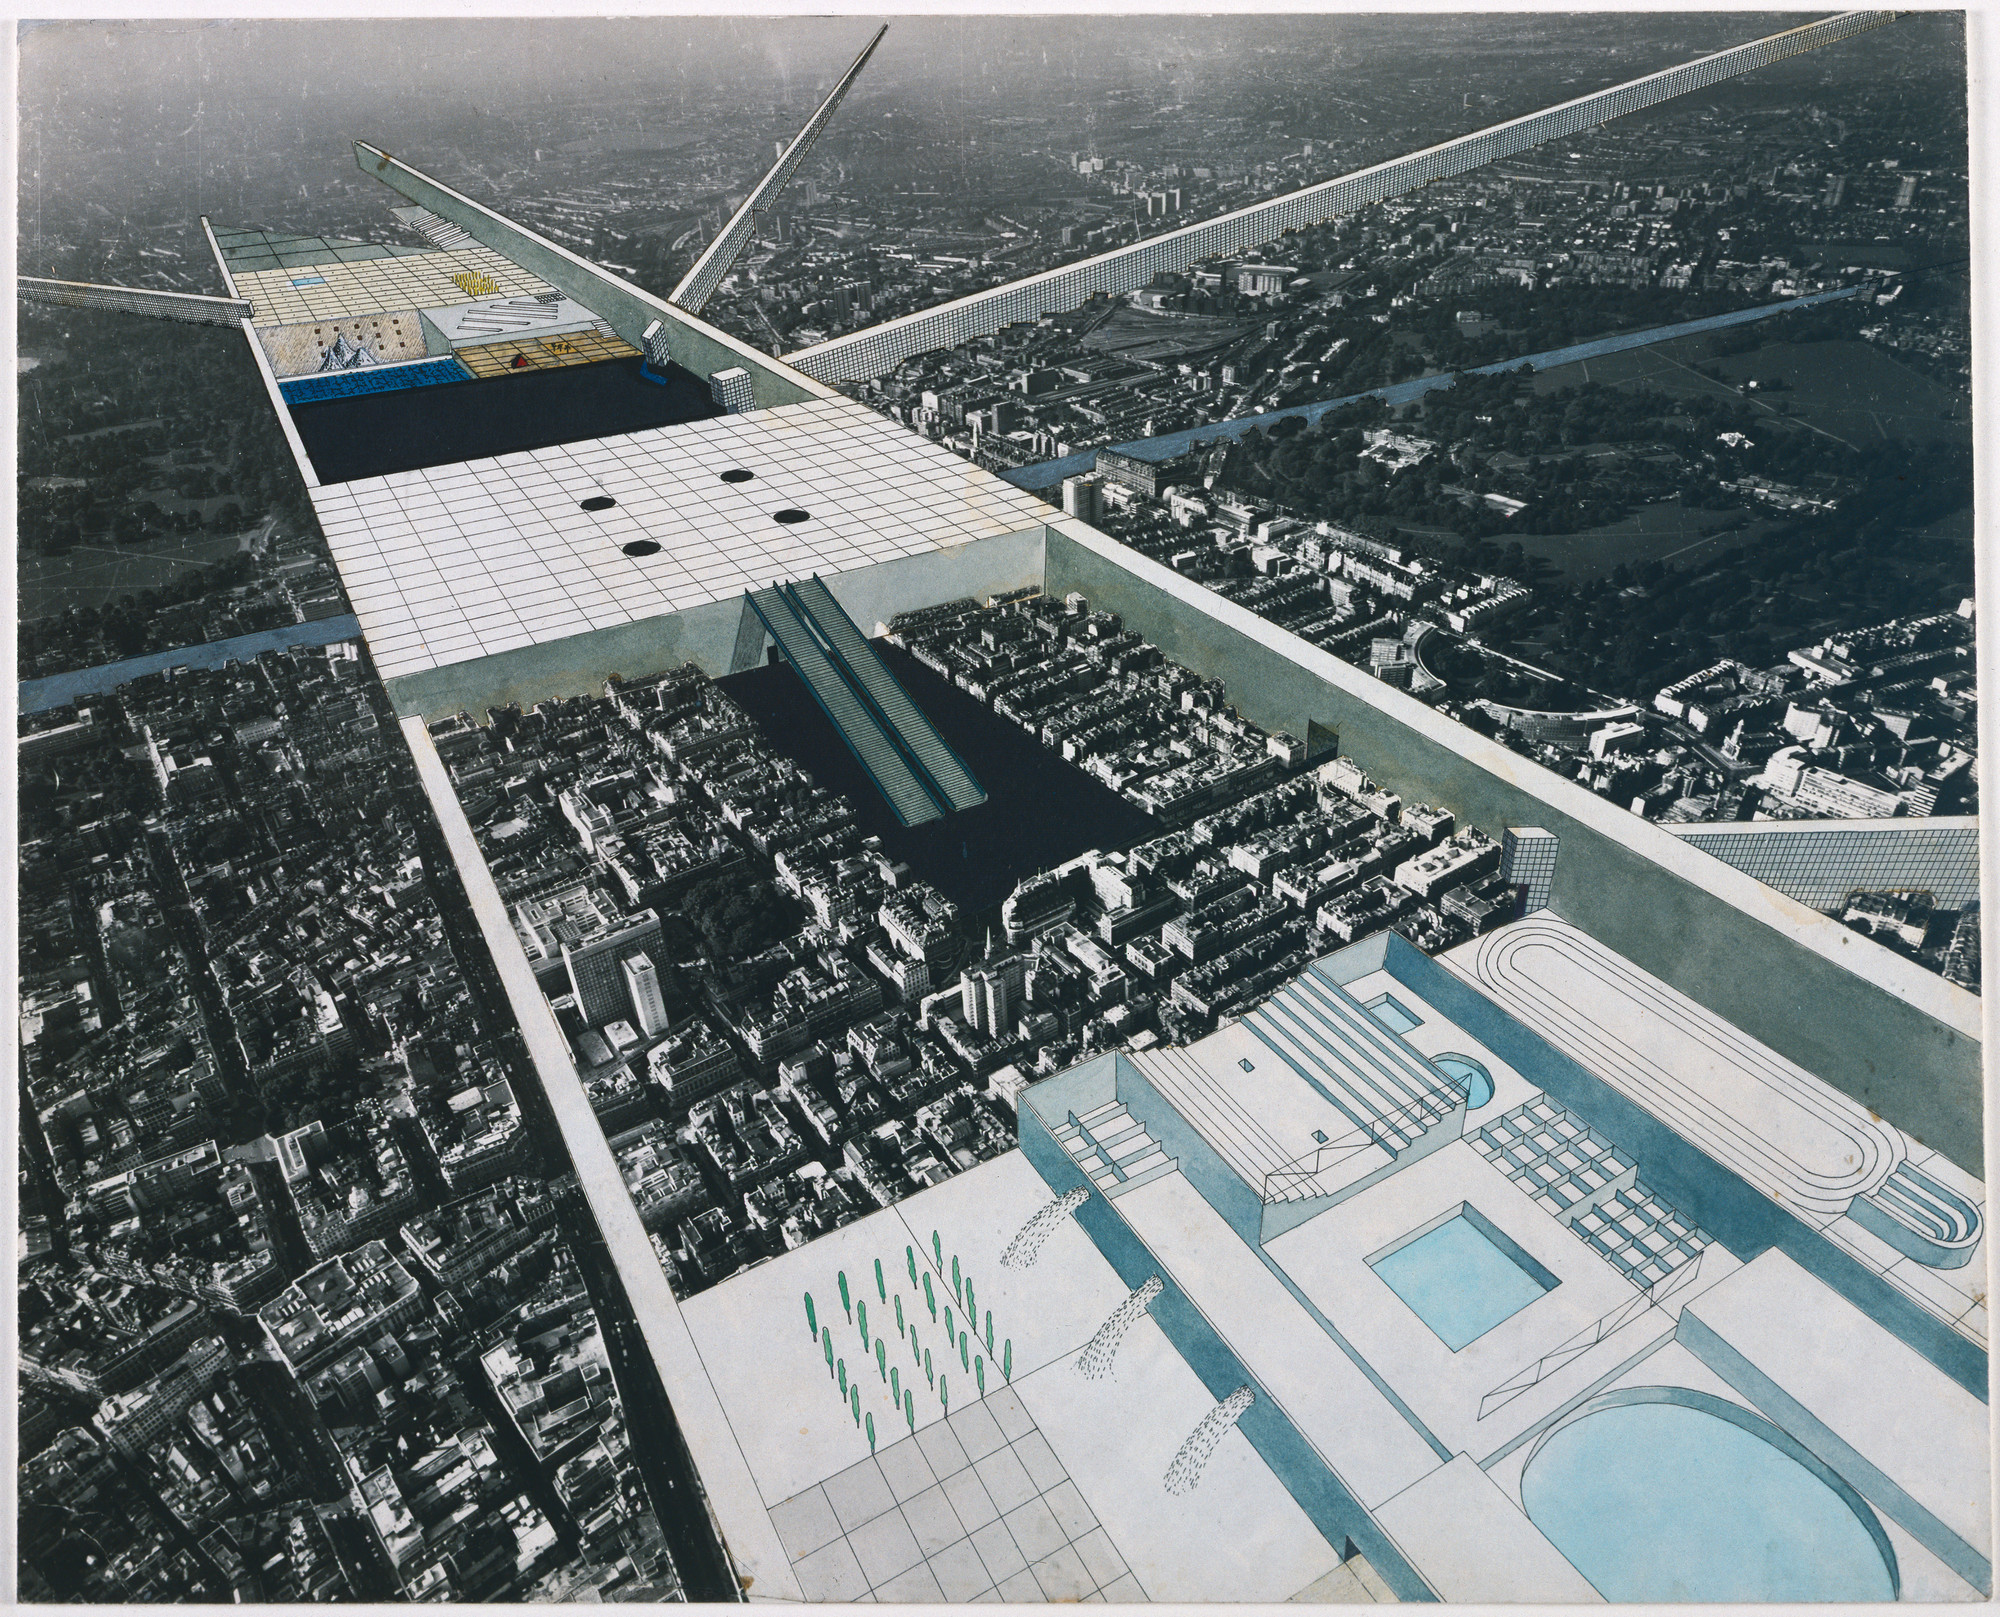
\includegraphics[width=0.7\textwidth]{chapters/fig/strip.jpg}\quad
\caption{``Exodus, or the Voluntary Prisoners of Architecture: The Strip (Aerial Perspective)''
by Rem Koolhaas, Elia Zenghelis, Madelon Vriesendorp and Zoe Zenghelis. The project
imagines a walled city of ``new urban culture'' within the city of London.}
% https://www.moma.org/collection/works/104692
\label{fig:exodus}
\end{figure}

The C\# Application Markup Language example hints at a number of themes that I will further
explore later. It is perhaps blatantly funny, but it can still be seen as making a serious point.
Moreover, the system that the post describes has never been actually implemented. The post
is merely a (very basic) plan for a system. This does not, however, make it any less valuable
as critical software. Many interesting pieces of critical architecture have also not been
built, yet, they became important references. The Chicago Tribune tower by Adolf Loos is one
such case, but even better example would be one of the many architectural projects that
use the architectural language to intentionally propose structures that cannot be built.
One such project is The Strip (Figure~\ref{fig:exodus}) by Rem Koolhaas. The project imagines
an enclosed restricted city cutting through London. Although the work was inspired by the
situation of West Berlin during the Cold War, the ideas of building a wall to separate cultures
can be seen in new (and alarming) light today.

In the subsequent chapters, we will see that hypothetical design proposals, fictional
plans that cannot be built or impractical systems are a powerful way of making a point
about software systems, just like they are a powerful way of making a point about architecture.
The C\# Application Markup Language can be seen an example of a much broader class of
esoteric programming languages, which are created jokingly, but can be often read as
valuable critiques.\endnote{Cox, Speaking Code}

\begin{figure}
\centering
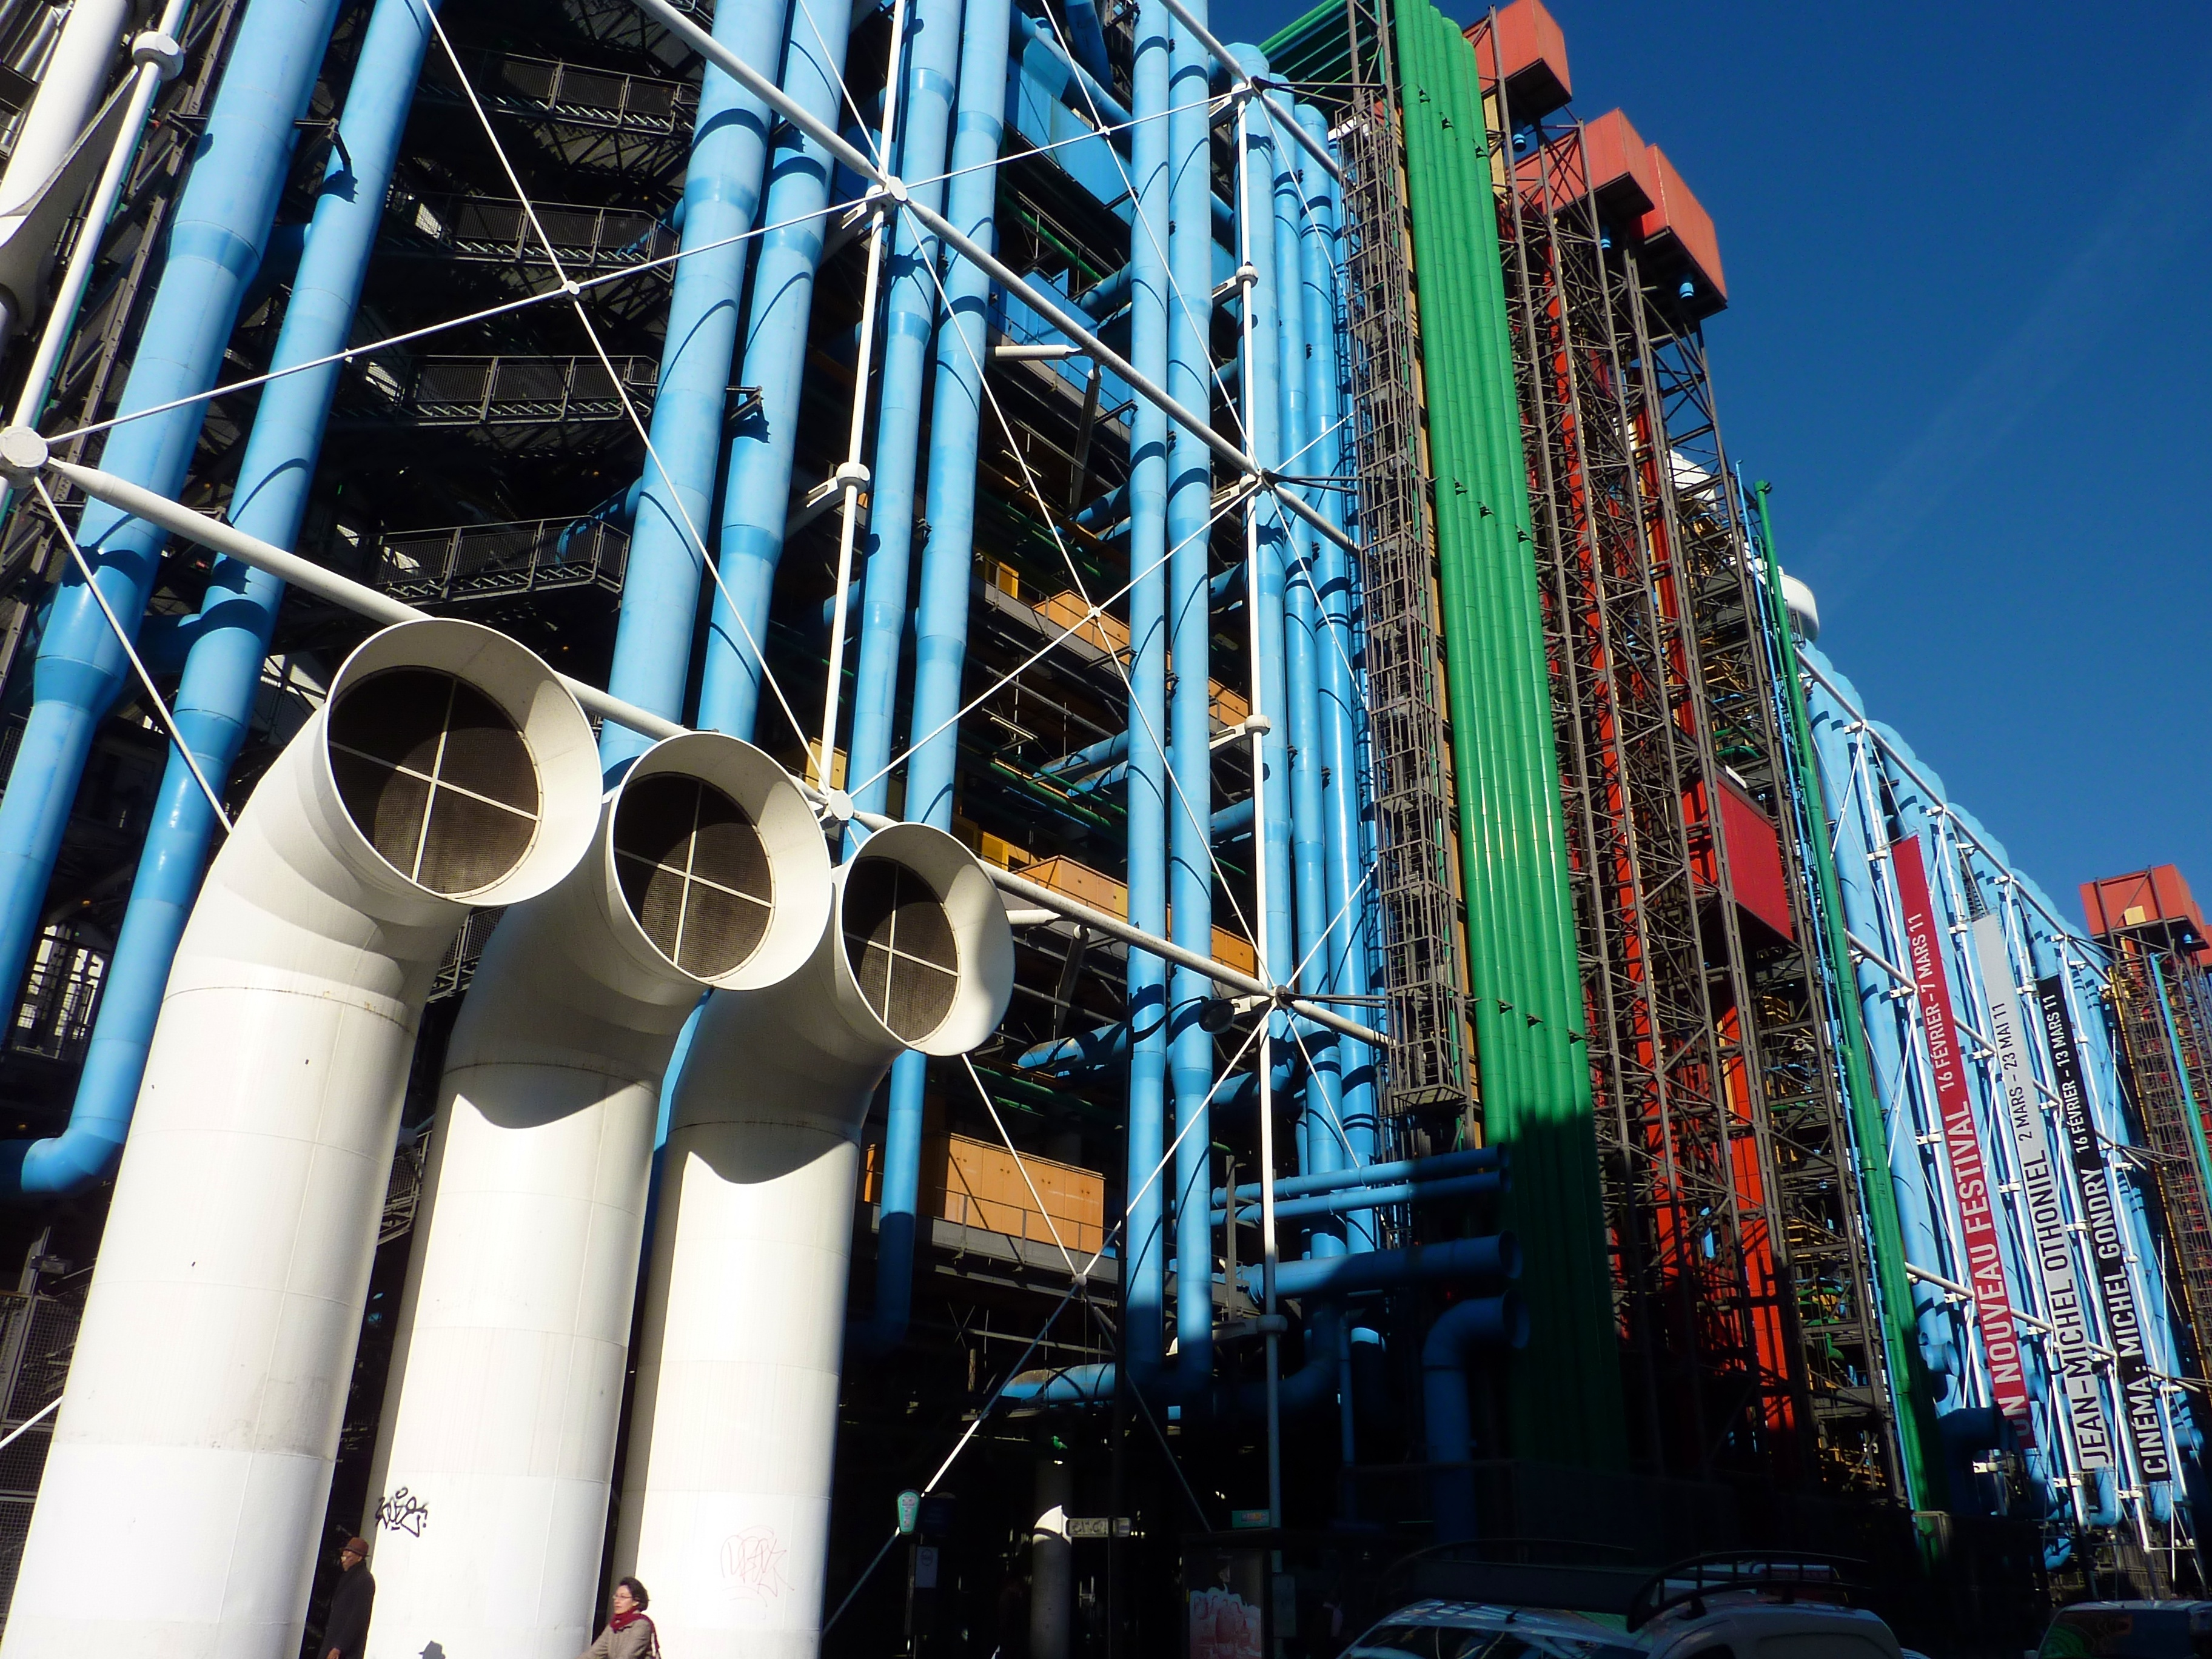
\includegraphics[width=0.85\textwidth]{chapters/fig/pompidou.jpg}\quad
\caption{The Centre Pompidou ``inside-out'' building, which keeps all the infrastructure
(using green for plumbing, yellow for electricity, blue for climate control, and red for
circulation) on the outside to allow flexible and efficient use of the inside space.}
% https://www.flickr.com/photos/jeanbaptistem/5448056975/in/photolist-HFZ9L-k5DdGP-9iqHwP-4vkacq-ydwXxD-9K2Jaz-k5LueV-k5Lh5K-HFYXU-ySUqb4-k5MyjB-ebvgdy-ydouoL-k5CwUF-9K2J1z-k5CV3R-2o6FcFX-m7tSj-aAbT1J-23edLxs-f9M6TH-k5CR2x-k5BJ4g-k5Cz5K-98pso6-4H9NcH-k5Q4fu-QMA3dr-4HdZ6y-aSKucT-4H9Nii-4HdYXd-6NgNR9-aSKC7P-74qk4S-4EvW6x-4fdBW2-9K2NKp-ebpE8F-z9o7SU-7yeN5y-byStES-a9DTqd-2qvg1Dn-ecAeV-nU1orA-bMM8zr-4EAaLQ-k5KdY6-4beX5c
\label{fig:pompidou}
\end{figure}

As I wrote earlier, I believe that we can take inspiration from the critical architectural
language both to analyze existing software systems and projects, but also to come up with
new ideas. Some of the references to a column that I discussed earlier make points that
may well be applicable to software systems. For example, they may ironically highlight the fact
that a column is used for its symbolic value, but not for its original purpose.
They highlight the fact that it is no longer needed functionally, even if it is often used
for rhetorical reasons.

We can imagine a range of similar critical points to be raised about the technical concept
of data structures in the context of programming and software systems. If a column is no longer
needed as a structural element, what may be the established essential aspect of data structures
that is no longer needed?

One of the most established ideas associated with structuring application data is that of
information hiding.\endnote{Parnas, On the criteria; also reflections in \url{https://link.springer.com/chapter/10.1007/978-3-642-59412-0_25}}
The argument is that one should separate software systems into components that have a stable
public interface and private implementation. If one identifies suitable stable public interface,
it is possible to develop the components in isolation, change the implementation or replace
individual components as needed. But information hiding has also been criticised.\endnote{GPII Nexus,
my article on architecture, Convivial Design Heuristics for Software Systems} The problem is
that predicting what part of the interface should be fixed and what can be hidden is often
difficult, especially in the context of software systems whose function evolves and changes
over time. Clark and Basman\endnote{GPII nexus} quote the example of MIDI SysEx messages that
have, by convention, become a mechanism that exposes the state and can control the operation
of musical devices. This enabled MIDI to become a powerful music control platform in a way
that could not have been anticipated by the designers of the MIDI interface in the 1980s.
Arguably, an even more prominent example would be the web platform, where much of the data
structures that the web is built around (HTML, CSS) are also transparent.\endnote{But this
has limits, see my talk.}

So far, most ciritiques of information hiding have taken the form of text. To make the point
through the critical language of software, we should design an exemplar piece of software
or programming system that reverses the idea of information hiding. In other words, we
should expose all the underlying data structures of the software in a way that is akin to how
the Centre Pompidou (Figure~\ref{fig:pompidou}) exposes all the service infrastructure of the
building.

In such hypothetical system,\endnote{suggested by Clark and Basman} all the state of the system
would be externalised in a way that allows anyone to see and modify it. To make the point,
the system should do this to the extent possible. The accessible state should include all
information about the data structures, as well as execution of the system. Depending on the
chosen programming paradigm, this may include data of all objects, memory, stack, currently
executing instructions etc. The information should also be exposed in a way that makes it
available not just to the programmer,\endnote{this is already possible via reflection or in
image-based systems} but also to the end-user. The system would have to handle the fact that
its state may be modified in inconsistent ways and could either recover as best as possible
(akin to how web browsers recover when encountering invalid HTML) or break (likely making an
interesting point about the fragility of software systems).\endnote{c.f. antifragile}
The color coding used in the Centre Pompidou offers another interesting idea. If we exposed
all data structures of a software system using similar color coding (for different aspects
of the system), the system would increase public awareness about what modern software consists
of. Thus the project can also fulfil an educational function.

There is, of course, a practical issue of the context in which such project can become
reality. It is entirely possible to develop a critical software system only in the form of
specification or description, much like Charles Petzold's C\# Application Markup Language.
However, to explore the consequences of the design---and see how a system can be used in
the absence of information hiding---an actual non-trivial working implementation is needed.
I will return to this problem later, but architecture has a variety of options. Many
architects explore their theories for houses built for their own use or their
family.\endnote{Gehry's residence, Vanna Venturi house} Similarly, programmers and computer
scientists often have their own projects to experiment on.

Architecture also often speaks through
non-building objects such as stage sets, public monuments, pavilons and follies or exhibitions.
Those may not (yet) have obvious equivalents in the world of software and the task of developing
critical language of software may involve finding those. Last but not least, new architecture
also sometimes emerges in isolated places within a large city, called heterotopias in reference
to Michel Foucault.\endnote{Jencks, 119} Such isolated spaces, such as prisons, ghettos,
amusement parks, or leftover spaces known as terrain vague.\endnote{vagni teren}
I believe we can similarly find a range of atypical pieces of software, which are often deemed
as unimportant, but provide space for experimentation. Ad-hoc scripts, demos, spreadsheets,
and programs created at hackathons or coding competitions are only a few examples of hterotopias
in the world of software.

% Oppositions p376
%
% "criticism embedded in practice" (Venturi) - not just code, but also docs
% Eclecticism - be funny (Jencsk) - engage with audience in a fun way?
% Morality / social relevance (Jencks) - c.f. thimbl
%
% self-referential sign
% -> thing ported from (native) environment to expensiove recreation in another? (to keep UX or something?)
%
% serious artists engage with history, choosing what to keep and what to drop (The Hub)
% rebuilding old things anew?
% -> reconstructions
%
% Class as a column?
% basic structure, associated with maintainability...
% (evolved from closures and back)
%
% god object / class? - chicago tribune
%
% types and data structures - in cases where they are not enforced (nosql) - mere nice annotations
% - data structure characerizes software - Craft, p96
% => vocabulary for what you can do - disrupt? nosql databases (allow anything) -
% c.f. craft p98 (disrupt the gap in definining vs. understanding SW structures?)
%
% point out things that we're doing without thinking (information hiding)
% -> expose structure
%
% Rhetorical element? (Venturi)
%
% highlight contradictions - plenty in software
% hard to read architecture is valid if it reflects contradictions (Venturi)
%
% exhibitions / stage sets
% -> format for communication
% -> heterotopias (Jencks)
%
%
% Deconstruction
% - use some methodological way rigorously to show where it leads

\newpage

\begin{figure}
\vspace{-1em}
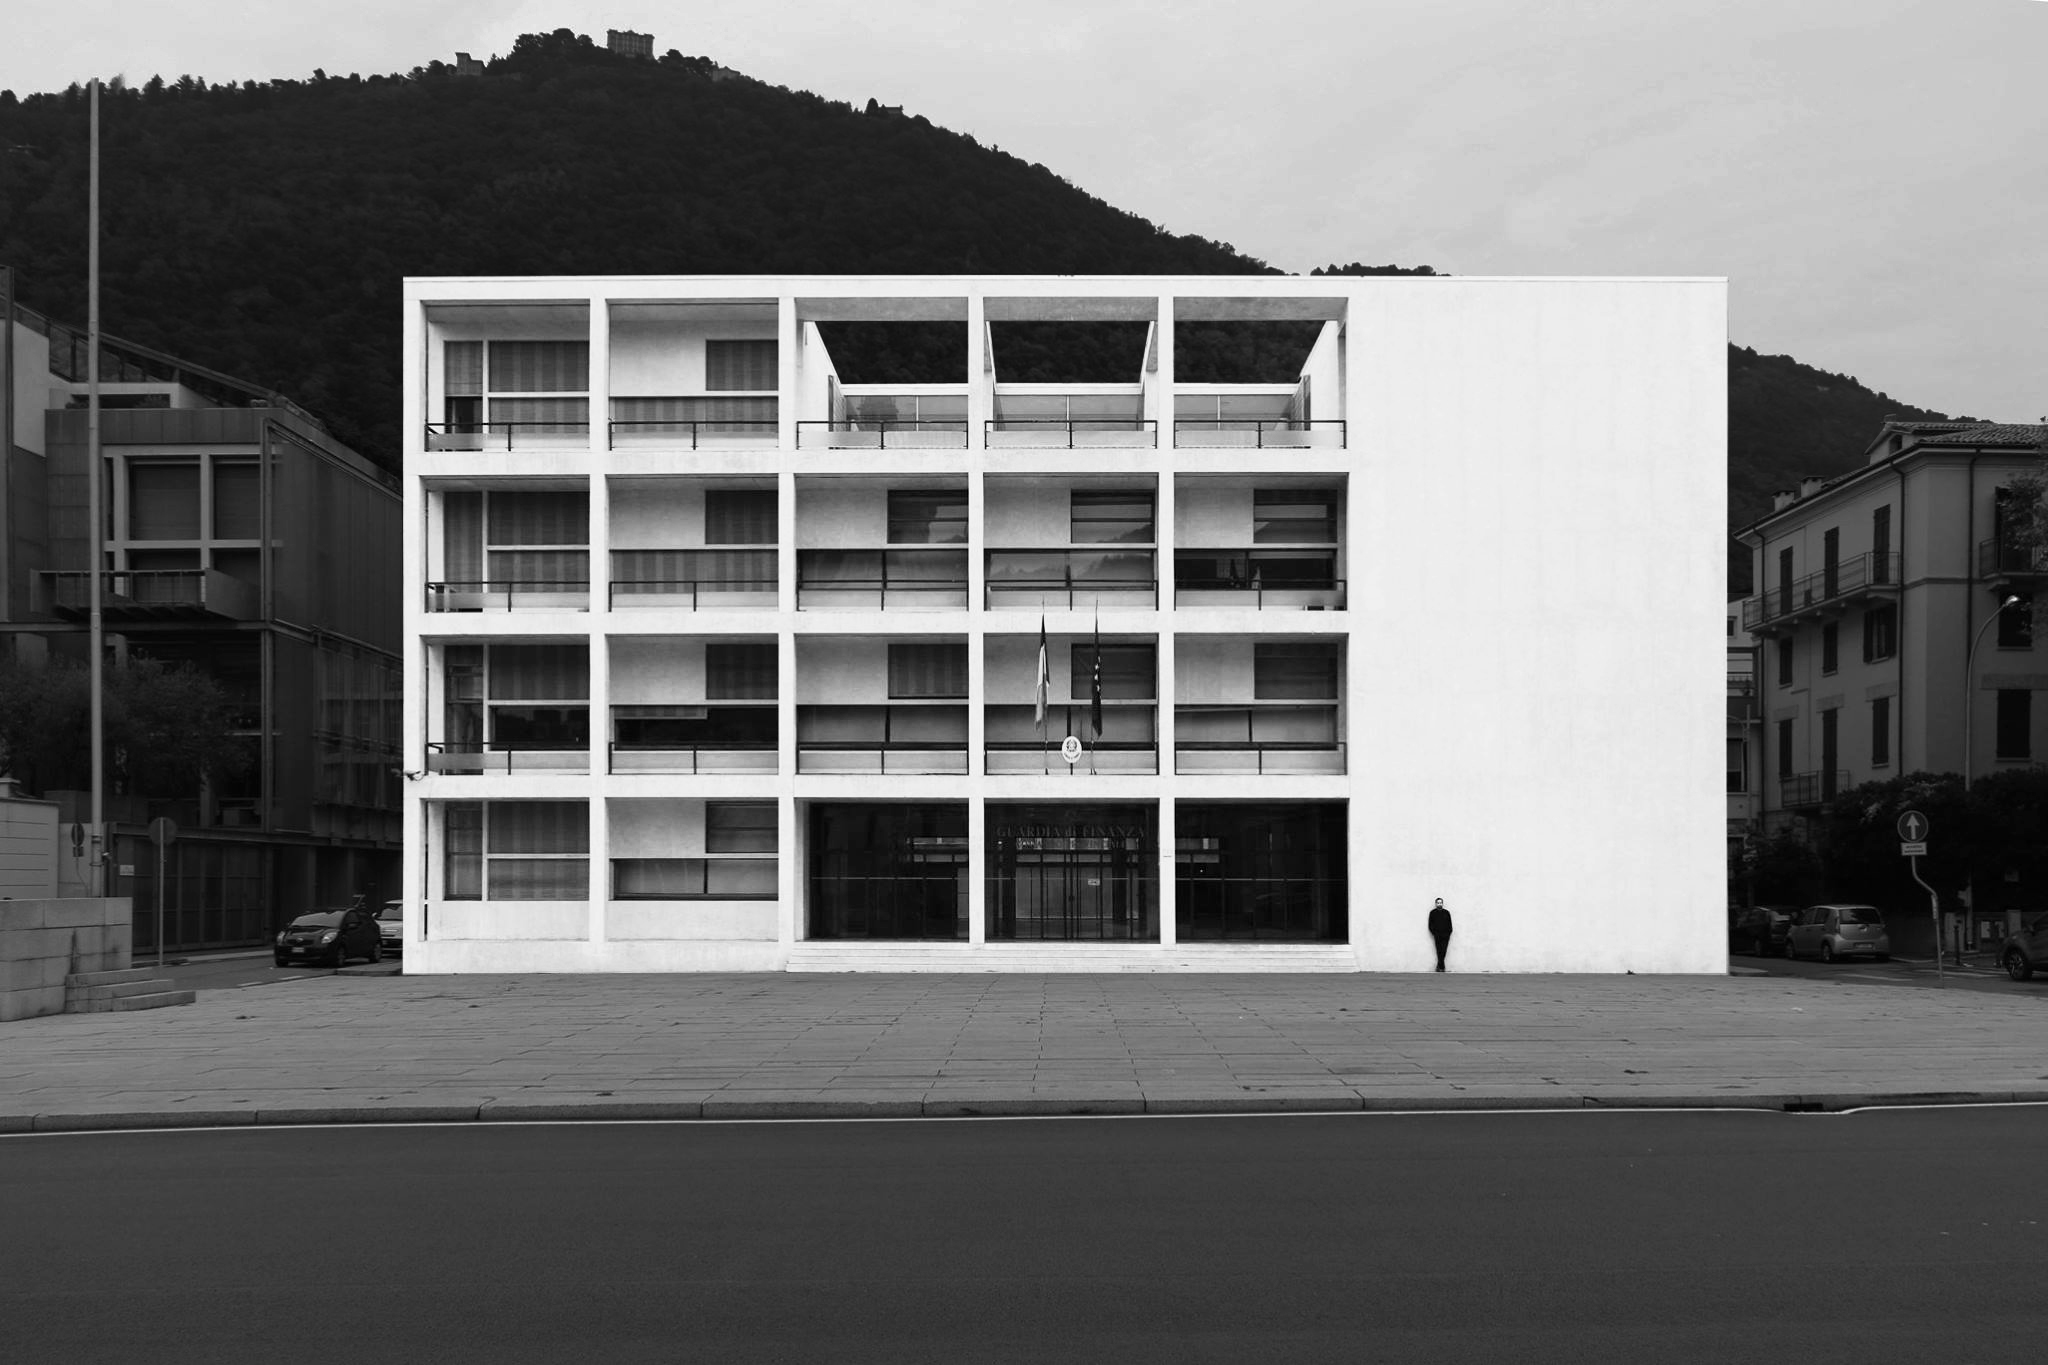
\includegraphics[height=8.5em]{chapters/fig/grammar-fascio.jpg}\quad
\raisebox{1.2em}{\boxed{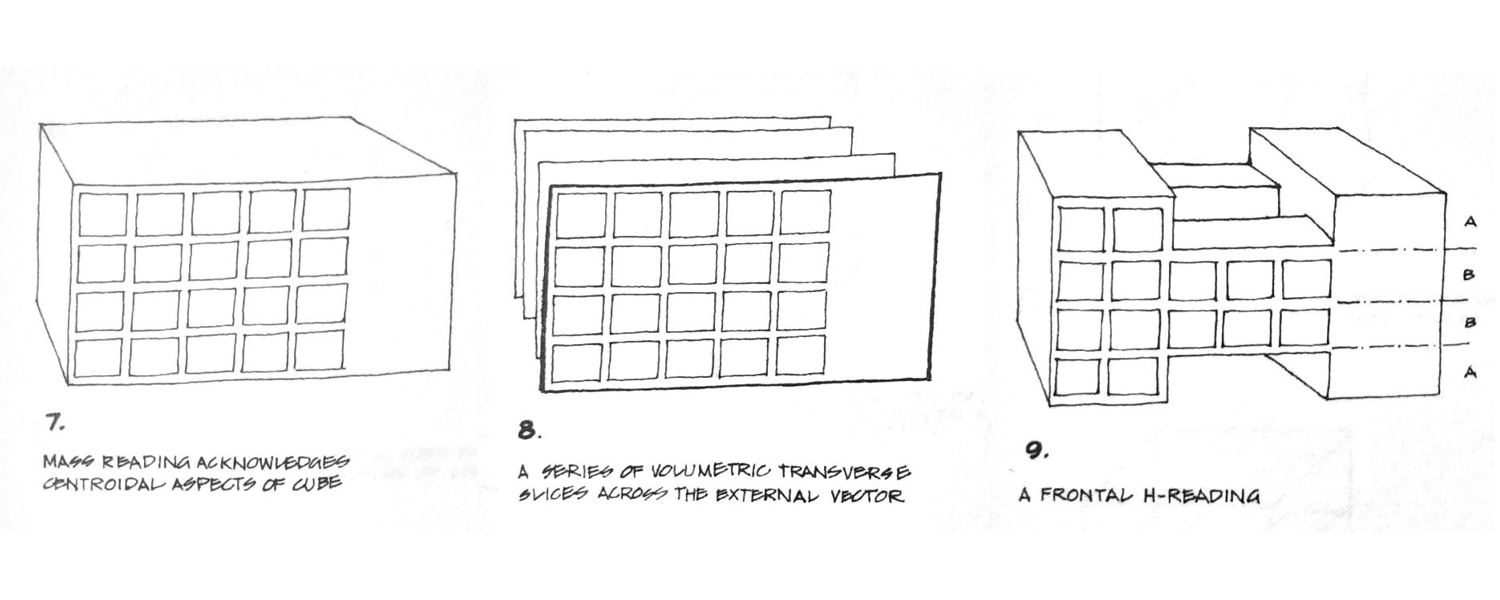
\includegraphics[height=7em]{chapters/fig/grammar-formal.png}}}\\[1em]
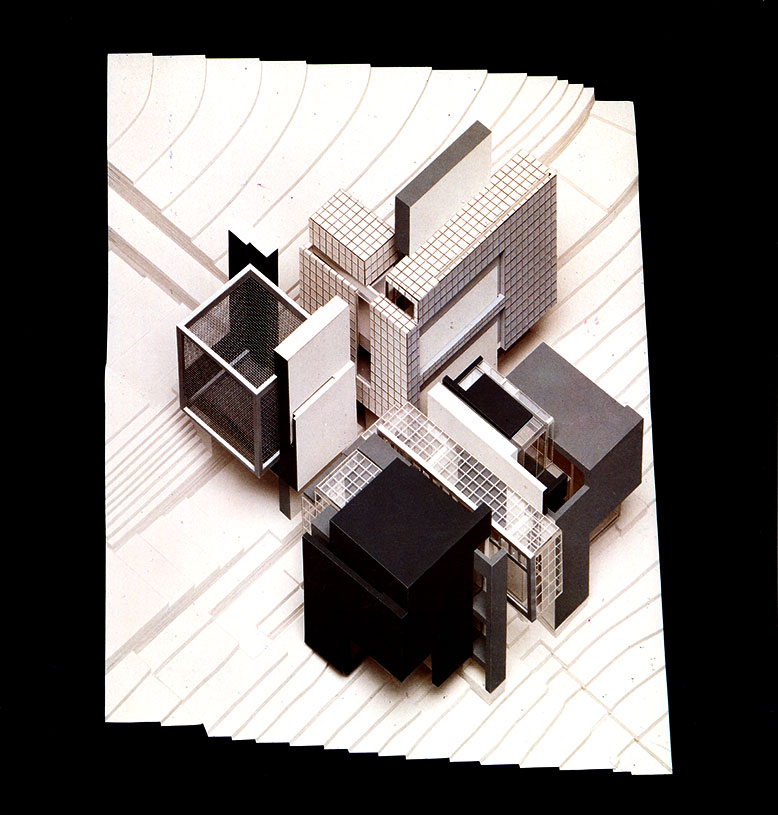
\includegraphics[height=9.5em]{chapters/fig/grammar-house-x-model.jpg}\quad

\includegraphics[height=9.5em]{chapters/fig/grammar-house-x-diagram.jpg}\quad
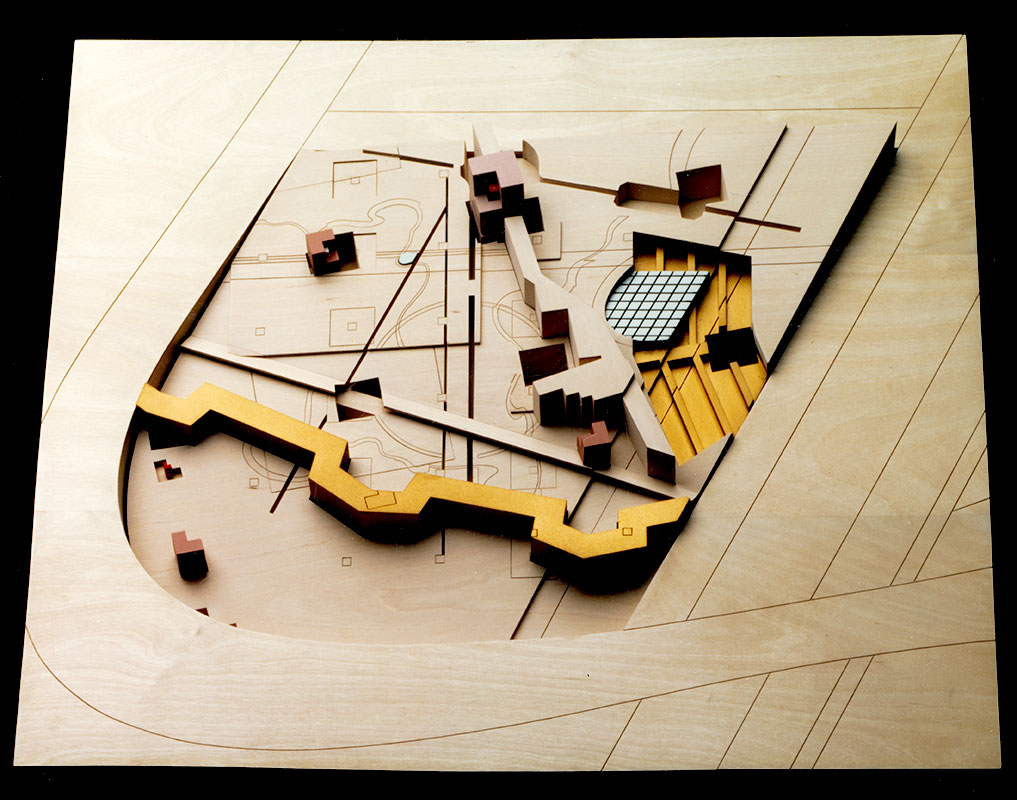
\includegraphics[height=9.5em]{chapters/fig/grammar-la-vilette.jpg}\\[1em]
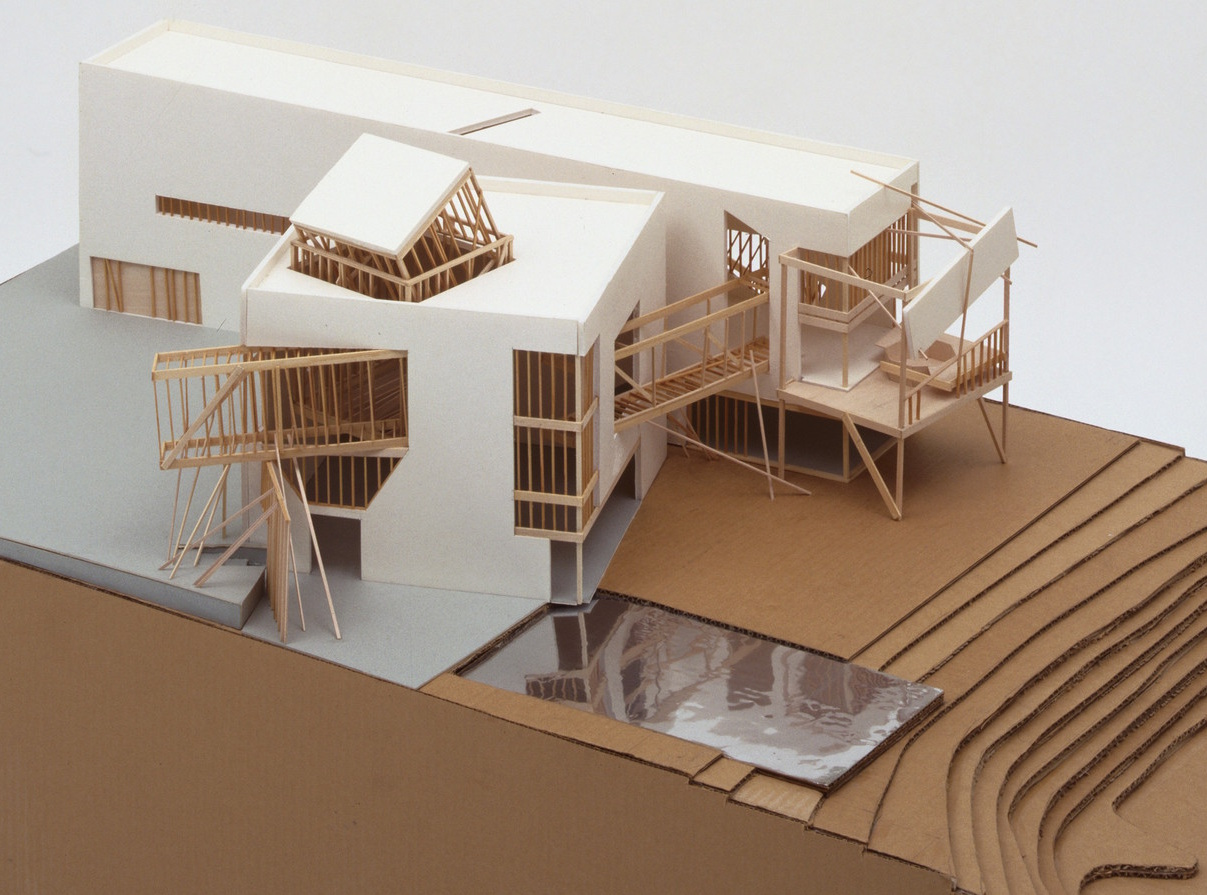
\includegraphics[height=11.1em]{chapters/fig/grammar-familian.jpg}\quad
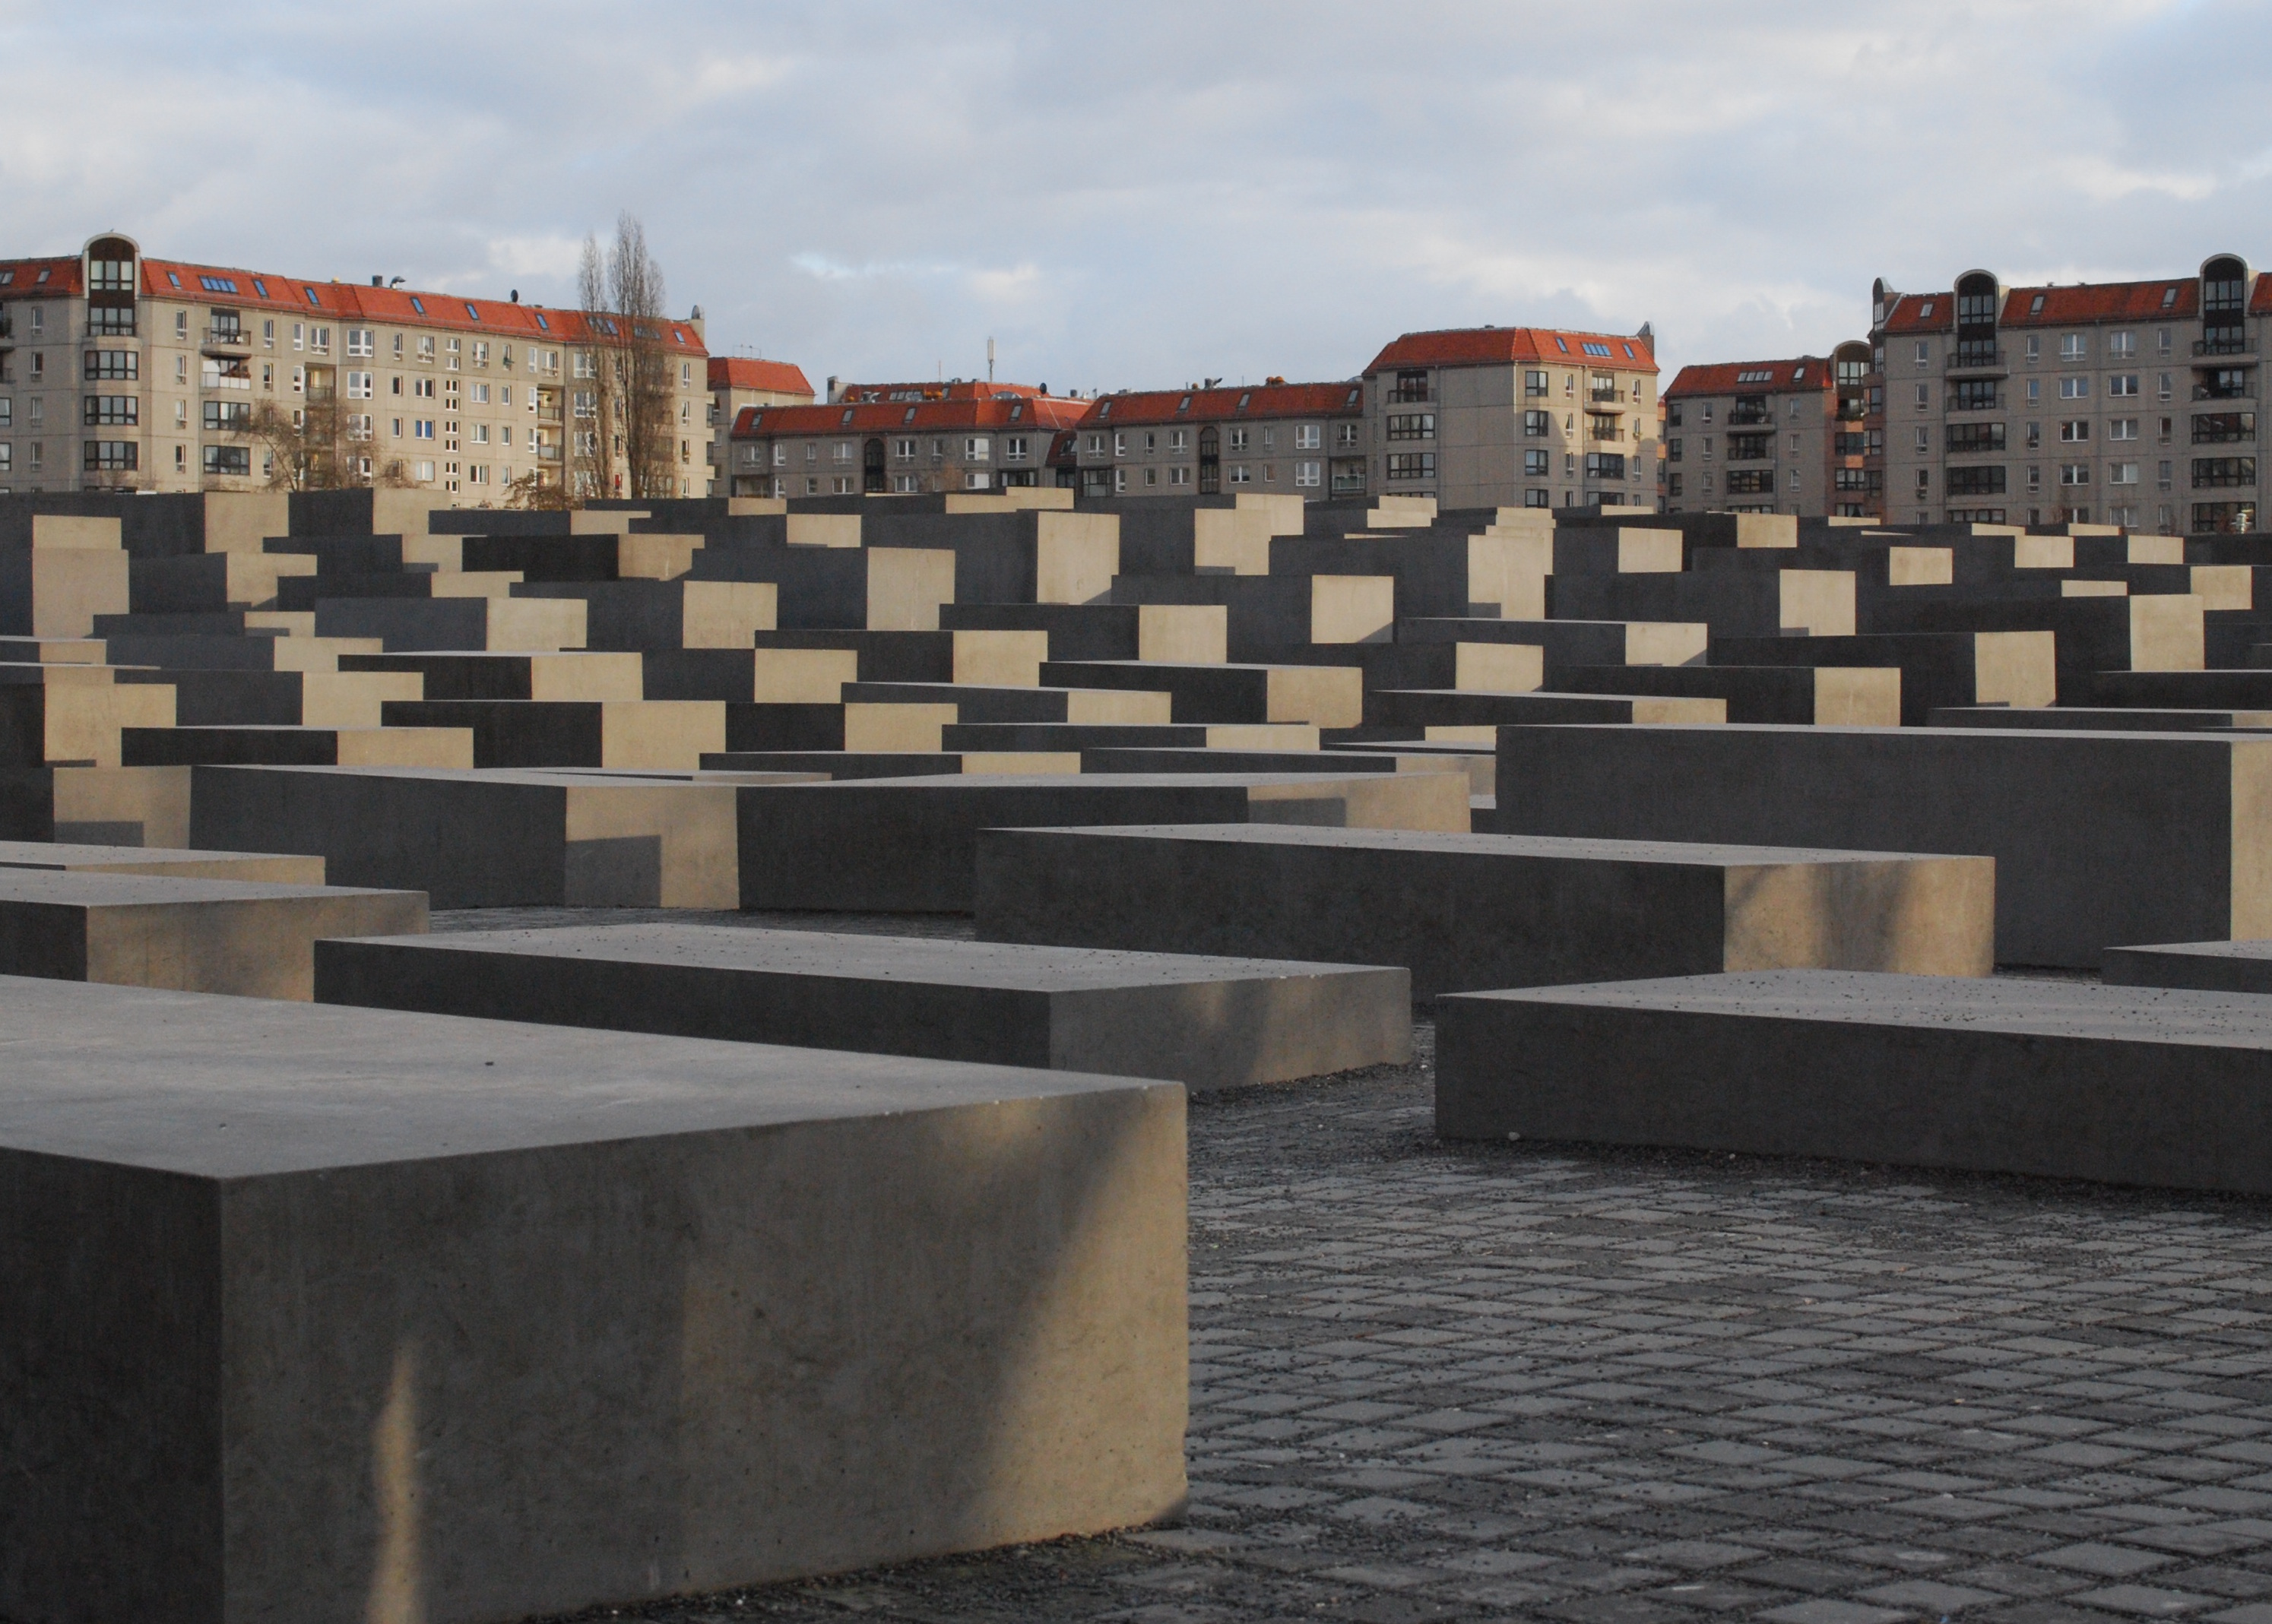
\includegraphics[height=11.1em]{chapters/fig/grammar-memorial.jpg}
% fascio - wikipedia
% memorial - (cropped) https://www.flickr.com/photos/kevingessner/3323686050/in/photolist-64GL4U-gmYANP-6YkWHE-8vUy7Q-9FH37x-pVsPse-5d4N58-2dVZT3p-67BAtZ-or2tXp-84DzeG-84AtzF-LtDWre-5rERP4-AWVNRW-2nV1U1m-CJngd7-5UyjuF-d1g2U-64GLH7-8bsffq-6YQqX6-gmXTZg-641dZT-2p9SPMP-61vkjE-64GLx5-64GLm7-8L4PSH-CJnfyb-qzFxwu-qZ3YXX-edtnMV-bsDTdV-8mgDe1-MsMXg8-7h3Fnw-8L4PZr-gmYrDQ-6ekCEq-ni4YuS-djLNZH-8L4Q6z-CXjdR-CJu3nH-74y5Mo-FshXT-D8opnP-2p4e5P-nhKtYg
% familian - https://www.moma.org/collection/works/1020 (cropped)
% la vilette - https://eisenmanarchitects.com/La-Villette-1987
\caption{Five different uses of what can be interpreted as a formal language in architecture.
(1)~Modernist Casa del Fascio in Como, Italy built in 1936 and (2) a formal analysis of the building
by Peter Eisenman, (3) model of the House X, also by Eisenman and (4) a diagram illustrating
its formal structure based on the L-shape, (5) model from a 1987 project for a garden in the
Parc de la Villette by Eisenman in collaboration with Jacques Derrida, (6) model of the unbuilt
Familian Residence house by Frank Gehry from 1978, and (7) the Memorial to the Murdered Jews of
Europe designed by Eisenman, completed in 2004.}
\label{fig:grammar}
\vspace{-0.5em}
\end{figure}

\section{Formal Grammars of Architecture}

In the previous two sections, I focused on ideas that approach architecture from
the particular, specifically the structural element of a column. I will now look at ways
of developing critical language for architecture starting from the general.
I look at a number of works, most notably by Peter Eisenman, that relate architecture to
language, art and their formal structures and grammars (Figure~\ref{fig:grammar}).

The most direct reference to formal grammar in the context of architecture comes
from Peter Eisenman's PhD thesis, completed in 1963 at University of Cambridge. His thesis,
``The Formal Basis of Modern Architecture'' is concerned with formal analysis of
form and formal order in modern architecture. Eisenman suggests that the architectural form
can be seen as a problem of logical consistency, rooted solely in the properties of basic
structures from which the architectural form arises. The view opposed that of modernists who saw
form as arising from function, as well as Christopher Alexander's view put forward in his
Notes on the Synthesis of Form.\endnote{see debate} In contrast with modernists:

\begin{quote}
Eisenmann saw modernist forms not as simple derivatives of functional needs, but as
delineations of the immanent self-referntial properties of architectrue itself,
as searches for objective knowledge that lies outside both the architural agent's intentions
and the building's uses, and inside the very materials and formal operations of
architecture.\endnote{Oppositions, x}
\end{quote}

The time was probably right for this kind of intellectual project.
Eisenman was influenced by his reading of the linguist Noam Chomsky,\endnote{Oppositions, 202}
who published his first work on formal languages and grammars at the end of the 1950s. The
same ideas also contributed to the development of formal grammars of programming languages at
the end of the 1950s.\endnote{Algol}

Eisenman's thesis is analytical. He considers the plans of a range of modern buildings,
including those by Le Corbusier, Mies van der Rohe and Alvar Aalto, and explains their
structure in terms of a number of simple formal principles. Those include three basic
kinds of movement systems throughout the building (pinwheel, spiral, echelon), three types
of volumetric systems (horizontal planes, vertical planes, plaid) and various interactions
between them that lead to distortions of and dislocations in the basic structure.

One building analyzed by Eisenman is the modernist Casa del Fascio in Como designed by
Giuseppe Terragni. Eisenman sees the formal structure of the building as the product of
``reconciliation between a centroidal plan and a linear site.''\endnote{Formal basis, p293}
The form is a hollowed out cube. The cube can be seen as a series of planes, which needs
to be acknowledged by the side facades and which imposes a connection between the front and
the rear facade. To accommodate access to the inner courtyard, which results from the centroidal
plan, the ``negative volume is then dislocated'' giving the frontal facade reading of
an H-form.

Eisenman's analysis may seem like a curious theoretical exercise, but architects who study
the structure or the langauge of architecture had a more fundamental objective. Their aim
was to establish autonomous architecture, that is architecture that ``opens the internal
processes of architecture to their own internal possibilities.''\endnote{Autonomy and the Will to
the Critical - Eisenman} In other words, they seek architecture that is not created in response
to various external forces (of which there are many), but that is rooted in its own basic
(necessary) principles.

Eisenman himself went on to explore various uses of a formal architectural
grammar, not just analytically, but also as the basis for new designs in his numbered series of
houses, some built and some unbuilt. The House X, for instance, is a critique of ``the idea of
development from simple to complex''\endnote{Oppositions, p219} by using the L-shape as the
starting point, replacing the conventional cube. The design questions the humanist ideology
by disrupting the centrality that is typical of most houses. Where one might expect a hearth or
a staircase, there is nothing. The fact that this introduces a degree of disharmony in the project
has become contentious issue. While, Eisenman argued that an importnat role of art and architecture
is reminding people that ``everything isn't all right'', Christopher Alexander in a debate said
that such design makes him ``incredibly angry'' and he saw projects that introduce disharmony
as ``fucking up the world''.\endnote{debate}

In the 1980s, the experiments with architectural language, its grammar and the decomposition
of architectural structures took another form. Influenced by the French philosopher Jacques
Derrida, architects started to use architectural language to question the basic structures
and their conventional meaning. Eisenman himself collaborated with Derrida on a
project for a garden in the Parc de la Villette. The proposal eventually developed\endnote{Chora L
Works} into a scheme that rescales and overlays a number of different structures including
historical state of the site when it was a part of city walls and other projects by Eisenman
and his collaborators.

The almost mechanical design method is used to destabilize traditional
values of architecture such as its human scale and function. The authors propose to do this by
making parts of the park unexpectedly large or small, or by making parts inaccessible.
The La Villette project thus uses the architectural language to question the basic assumptions
of architecture. The project, again, causes the kind of disharmony that would enrage Christopher
Alexander.

In a critical commentary on the Parc de la Villette, Jeffrey Kipnis explained that
the point of deconstruction is to ``battle with the very meaning of architectural
meaning.''\endnote{Kipnis in Chora L works, p137} Because ``deconstruction deconstructs the
homogeneity, the unity of style`` it cannot, according to Jacques Derrida yield to
a single architectural style. Yet, this is what, perhaps somewhat inadvertently, happened
in the 1980s when the theoretical works of Eisenman got jointly exhibited with more literal
or pragmatic works by architects such as Frank Gehry, Zaha Hadid or the Austrian firm Coop
Himmelb(l)au.\endnote{Deconstruction in Architecture, at Tate and Deconstructivist Architecture
at MoMA, both 1988.} % https://www.dezeen.com/2022/05/20/deconstructivism-architectural-design-magazine-andreas-papadakis/

An early example of what became known as deconstructivist architecture is the series of Frank
Gehry's residential designs of the late 1970s and early 1980s. Gehry's work combines
experiments with different materials and spatial dynamics with the rejection of the modernist
grid.\endnote{See Frank Gehry, Architect: The Art of Architecture (Guggenheim Museum Publications)}
His formal structures are inspired less by grammars of Chomsky, but by avant-garde artists.
For example, the ``main masses [of his Familian Residence house] form a clearly Supermatists
grouping, recalling Malevich's Red Square and Black Square.''\endnote{The secret life of buildings:
An American mythology for modern architecture}
As noted by Charles Jencks, ``Gehry’s method of Deconstruction can be quite literal at
times, since he will smash an existing building into parts, leave elements of his own work
unfinished and (...) make an aesthetic virtue of rough, crumbled surfaces.''\endnote{Deconstruction
in Architecture (Papadakis, ed.) - p18} Yet, despite the different aesthetic and conceptualization
of the work, there is a clear connection between the work of Eisenman and Gehry. In some of their
works, they both try to uncover basic forms that comprise architectural structures and reveal them
through distortion.

The formal abstract structure, resulting from the composition of primitive architectural forms,
was also the basis for Eisenman's design for the Memorial to the Murdered Jews of Europe,
also known as the Holocaust Memorial in Berlin. The same formal mechanisms that were used as
a critique of humanism in architecture are used to create an unnerving experience for the
visitor.\endnote{Callaghan, M. (2020). Empathetic Memorials. Palgrave Macmillan Memory Studies.}
The abstract form of the memorial, devoid of symbolism and narrative, ``grants no further
understanding, since understanding the Holocaust is impossible.''\endnote{\url{https://eisenmanarchitects.com/Berlin-Memorial-to-the-Murdered-Jews-of-Europe-2005}}
In other words, the Holocaust Memorial is a structure that calls exactly for the kind of
disconcerting disharmony that Eisenman explored in his early house designs. According to
a brief explanation provided by Eisnman:\endnote{\url{https://eisenmanarchitects.com/Berlin-Memorial-to-the-Murdered-Jews-of-Europe-2005}}

\begin{quote}
This project manifests the instability inherent in what seems to be a system, here a
rational grid, and its potential for dissolution in time. It suggests that when a supposedly
rational and ordered system grows too large and out of proportion to its intended purpose,
it loses touch with human reason. It then begins to reveal the innate disturbances and potential
for chaos in all systems of apparent order.
\end{quote}

The formal architectural language explored by Eisenman since the start of his career thus
finds a new kind of use in the memorial. As with the Facade of Morphed Columns for the Venice
Biennale, the Holocaust Memorial is a different kind of architectural place, or a heterotopia,
where different architectural language can be, and needs to be, explored.

%
% circular houses, external storage; move to private rectangular houses with storage
% move to private houses (Aureli p88)
%

\begin{figure}
\centering
\vspace{-1em}
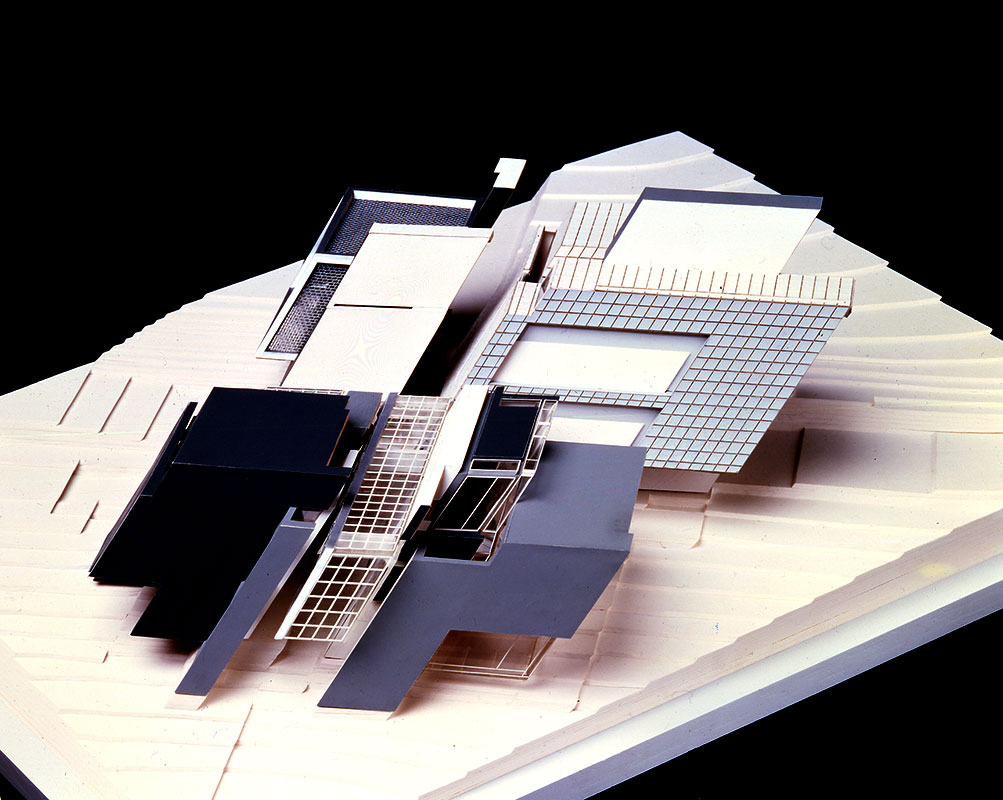
\includegraphics[width=0.65\textwidth]{chapters/fig/axonometric.jpg}\quad
\caption{Axonometric model of House X, which is a three-dimensional construction,
made to provide the image of a two-dimensional drawing from one particular angle.}
% https://eisenmanarchitects.com/House-X-1975
\label{fig:axonometric}
\end{figure}

\section{Questioning the Structure of Software}
Architects who probe formal structures of the architectural language may do so to better understand
the language, uncover assumptions that we accept and rarely question and explore consequences of
changing or manipulating the language. As in the previous section, this is often done using the
architectural language itself. Eisenman's numbered series of houses, Ghery's residences and Parc
de la Villette were all planned to be built and a number of them still stand.\endnote{And even houses
built to question the humanist focus of architecture sometimes found their satisfied owner.
\url{https://www.nytimes.com/2002/10/10/garden/house-proud-a-white-elephant-reincarnated.html}}
This fact, again, points at the possibility of a critical language that is not external to the subject
matter, but integrated within it. That is, the use of architecture to make critical architectural points
or, in the case I am interested in, the use of programming and software to make critical points about
software.

In some cases, architects use other formats too. Eisenman's doctoral work was a text presenting
a formal analysis of existing buildings. The deconstructivist practice can be used to probe the
process of architecture as well, as well as other artifacts it involves. For example,
another way in which Eisenman criticises humanist ideology of architecture is the
axonometric model of the House~X (Figure~\ref{fig:axonometric}), which makes
``the `normal' image appear to be an anomaly.''\endnote{Oppositions, 219}
Similarly, computer scientists and programmers should include a broader range of materials in
their notion of critical language of software, including formal definitions or software
specifications. Those can, no doubt, be constructed in a similarly illuminating distorted
manner as Eisenman's axonometric model.

The analytical way of looking at basic structures of the language of the subject matter is something
that computer scientists are well familiar with. It has been done at multiple levels. On one
level, formal models of computations such as Turing machines and the lambda calculus have been
used to describe the basic structure of computation. Like the grammar that reduces architecture
to relationships between basic shapes, formal models of computation reduce program execution to
a minimal set of operations. That said, there is a difference between computing and architecture
here in that formal models of computation originate in logic and have been conceived to study
computability properties, rather than actual program execution.

\begin{figure}
\centering
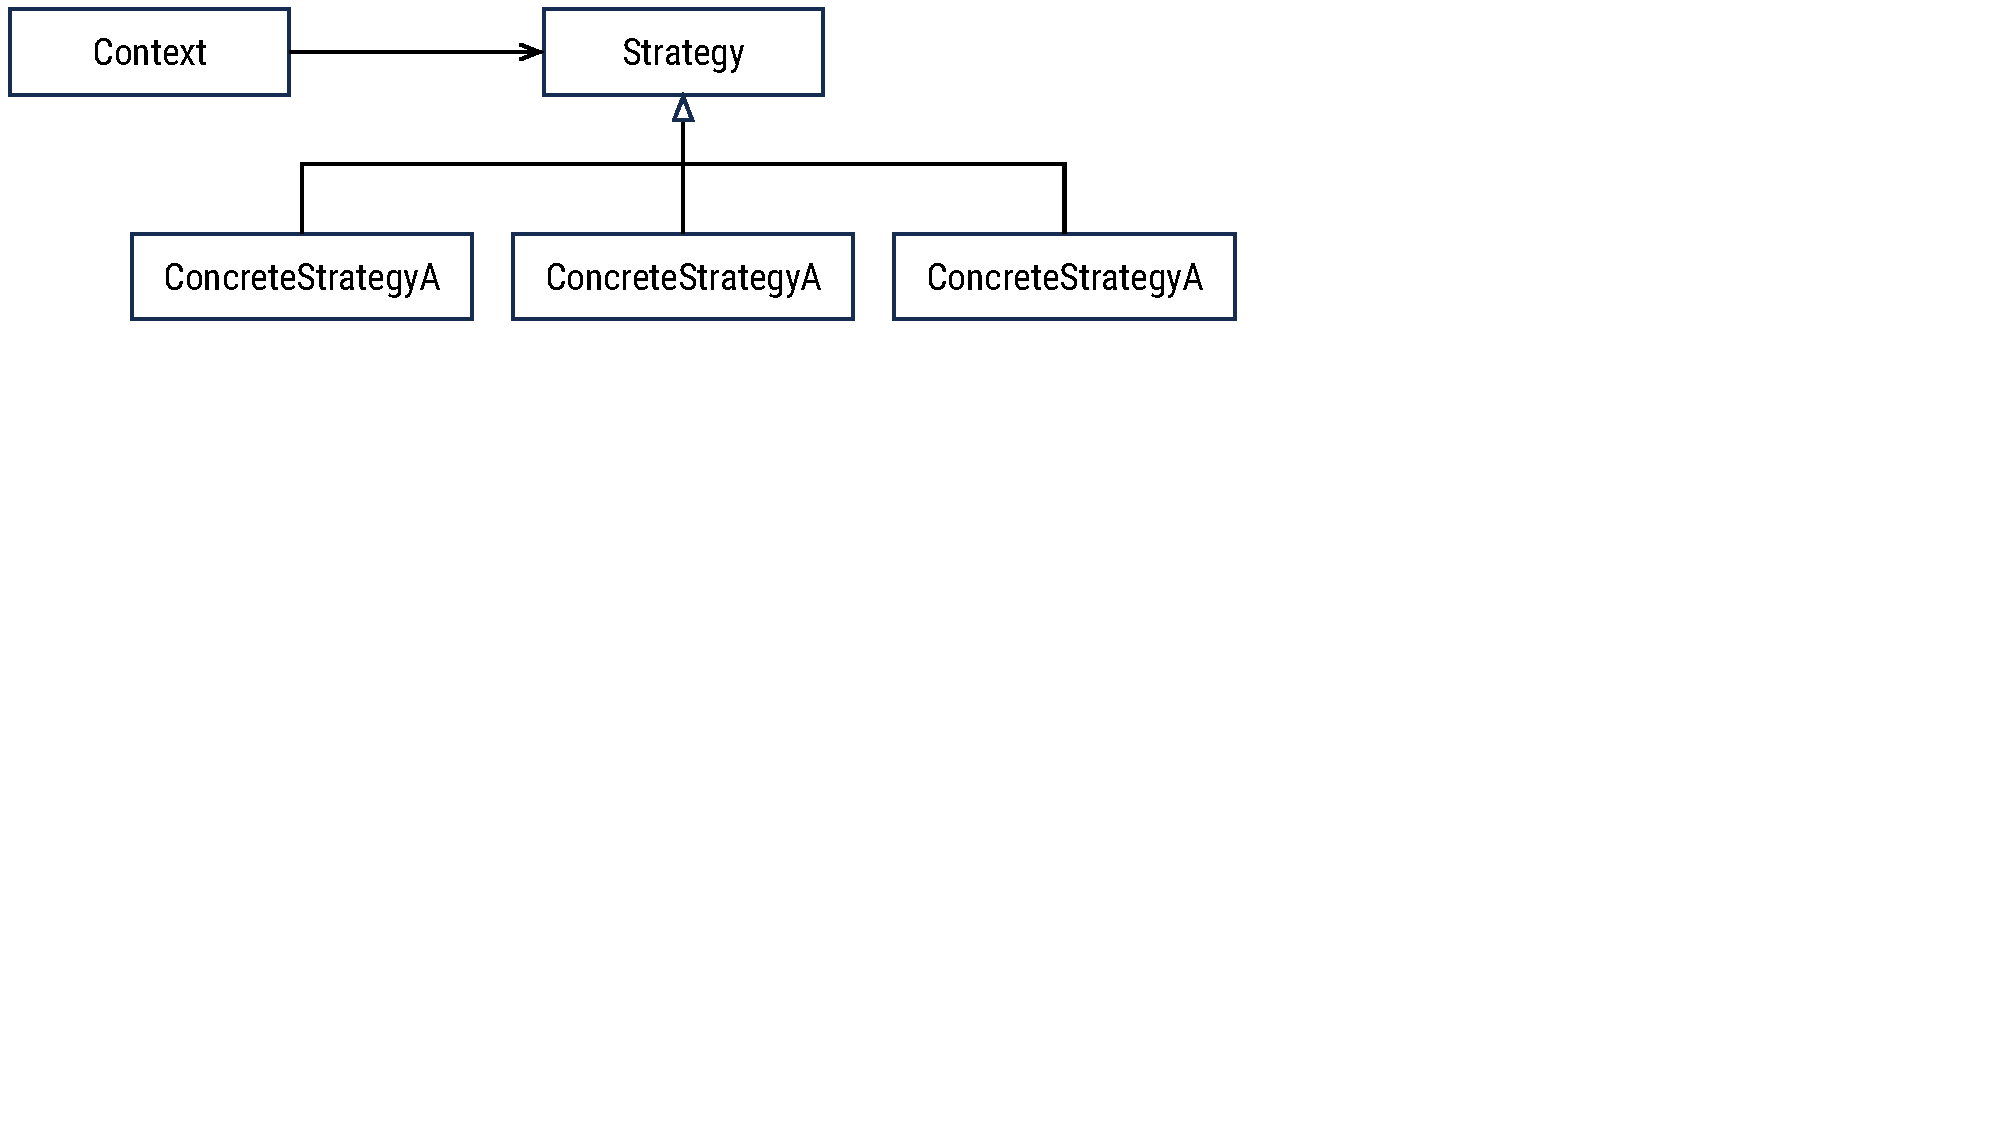
\includegraphics[width=0.7\textwidth,trim=0cm 13.5cm 12.5cm 0cm,clip]{chapters/fig/strategy.pdf}
\caption{A class diagram illustrating the relationships between classes and interfaces in the
case of the Strategy design pattern. The Context class uses a Strategy to do some work and
there is a number of specific strategies that can be supplied to it.}
% own
\label{fig:strategy}
\end{figure}

We can interpret software design patterns as another attempt to uncover the basic
structure of software. The influential Gang of Four design patterns book\endnote{cite} identifies
and catalogues some 24 design patterns, which appear repeatedly in past software systems. The
patterns are common structures defined by relationships between classes and interfaces in an
object-oriented systems and each design pattern captures one particular structure
of relationships (Figure~\ref{fig:strategy}). Although the Gang of Four book is a collection of
a larger number of patterns whereas Formal Basis of Modern Architecture is more akin to a formal
grammar, they are both similar in that they analyze existing systems (software or modern
architecture) to identify and describe their formal underlying structure.

Linking software patterns to Eisenman's work is ironic in that Alexander and Eisenman saw
their approaches as being in direct opposition,\endnote{debate} but I believe this may be
revealing. Whereas Alexander focused on creating ``living structures'', Eisenman is looking
for ``formal structures''. The Gang of Four design patterns are sometimes criticised for lacking
this essential ``living'' aspect emphasized by Alexander. The notions that Alexander has been
looking for are more likely to be found in the work of Richard Gabriel\endnote{Patterns of Software}
than in the widely used Gang of Four patterns.

On another level, there have been attempts to analyze and describe how software is made of
high-level concepts, which are rooted in the specific domain that the software is designed
for. In a book titled ``The Essence of Soware'',\endnote{cite} Daniel Jackson views software
as collection of interacting concepts. As an example, concepts involved in a social media
platform like Facebook include that of a post, comment, like and a friend. The exact structure
and interactions between such concepts then determine how the system behaves, how it can be
used and also its social implications.\endnote{Twitter and tear gas}

All of those formal structures in software---models of computation, design patterns and
concepts---can be used as analytical tools for understanding and analysing existing software
as well as help programmers in creating new things. You can use models of computations as a
basis for a new language, patterns to design an extensible software system or concepts to
create an intelligible application.

An important lesson that post-modern architecture teaches us is that we can use such formal
structures also to reveal the insufficiencies in our established practices, question hidden
assumptions or reveal the contradictions often present in software desing and development.
To paraphrase Eisenman, (admit and) show that everything is not all right. The illustrations
shown in Figure~\ref{fig:grammar} and discussed in the previous section suggest some ways
in which this can be done. We can use formal structures in a more or less distorted way,
follow a methodology in an excessively rigorous way, or start with atypical arrangements
of the basic structures.

I doubt there are many designers of programming languages who have studied work of post-modern
and deconstructivist architects and then decided to design a programming language according to
the same principles. But if we look at some existing programming languages, we can imagine what
this might look like. If we decide to use the lambda calculus as our primary model of computation,
there are multiple ways in which this formal structure can be turned into a programming language.
If we want to take the core structures of the formal model (variables, lambda functions and
application) and build a programming language around them, we have to bridge a large gap.
A realistic programming language will need much more than basic three primitives. Languages like
Haskell resolve any design concerns that arise from this gap using a reasonable programmer's
intuition---they aim at building a practically usable system.

It is certainly also possible to use the same formal model of computation and highlight the fact
that what remains to be added in order to design a practically usable programming language is by
no means obvious. One illustration of this is the esoteric programming language
Unlambda\endnote{some kind of citation} created by David Madore. The language is based on a
combinatory logic that is related to the lambda calculus and expresses computation in terms
of three primitive combinators written as S, K and I. Unlambda turns the formal model into a
programming language that makes it possible to write and execute programs, such as the following
Fibonacci number calculator:\endnote{\url{http://www.madore.org/~david/programs/unlambda/}}

\begin{lstlisting}
```s``s``sii`ki
  `k.*``s``s`ks
 ``s`k`s`ks``s``s`ks``s`k`s`kr``s`k`sikk
  `k``s`ksk
\end{lstlisting}

Unlambda supports a number of further functional programming concepts including continuations
and lazy evaluation. The \texttt{.*} construct prints the \texttt{*} character and returns it.
Unlambda is an ironical demonstration, not intended for practical use. Yet, it brings to light
a fact that is not otherwise easy to see. If we contrast Haskell and Unlambda,
we can see how much of the design of the Haskell language is not determined by its core
formal computational model---an interesting lesson about programming language design!

\begin{figure}
\begin{lstlisting}[language=csharp]
static class YCombinator<T, TResult> {
  private delegate Func<T, TResult> RecursiveFunc(RecursiveFunc r);
  public static Func<Func<Func<T, TResult>, Func<T, TResult>>, Func<T, TResult>> Fix
    { get; } = f => ((RecursiveFunc)(g => f(x => g(g)(x))))(g => f(x => g(g)(x)));
}

static class Program {
  static void Main() {
    var fac = YCombinator<int, int>.Fix(f => x => x < 2 ? 1 : x * f(x - 1));
    var fib = YCombinator<int, int>.Fix(f => x => x < 2 ? x : f(x - 1) + f(x - 2));
    Console.WriteLine(fac(10));
    Console.WriteLine(fib(10));
  }
}
\end{lstlisting}
\caption{Program that calculates factorial and Fibonacci numbers, unnecessarily overusing
the core concepts of the lambda calculus (fixed point operator) rather than relying on
standard capabilities of the C\# programming language.}
\label{fig:ycombinator}
\end{figure}

Last, but not least, we can also explore the case that integrate primitive structures from
multiple formal models of computation. For example, many programming languages that are based
on different principles (such as imperative, object-oriented languages) now support the
key concept from the lambda calculus, that is a lambda function. (Incidentally, this replaces
the Strategy design pattern illustrated in Figure~\ref{fig:strategy}.) Such combination of
different formal structures poses a problem both for language designers and language users.
The designers have to resolve the contradictions that arise from the integration of different
formal structures. (The complexity of the capture clause in C++ lambdas would be one example
of this difficulty.\endnote{\url{https://learn.microsoft.com/en-us/cpp/cpp/lambda-expressions-in-cpp}})
At the same time, the users of the language now have to carefuly choose between the multiple
available formal structures. Using ironical example, such as the two recursive
computations in C\# shown in Figure~\ref{fig:ycombinator}, we can point out that such choice
is not always easy. Somewhat like Ghery's residential projects, the example ``smashes'' together
parts of the programming language, making an aesthetic virtue of ``rough, crumbled'' lines of code.


~

~

CAVEAT - only programmers see this

two more at conceptual level - impossible UX, ads in facebook

%

~

~


* interpreting
  ??
    C\# lambdas - maybe distorted
* pure form
    lambda calculus
* distorted
    impossible UX
=> show that everything is not OK
* follow mechanical process (ad absurdum?)

Jackson-like concept analysis - but applied to real structure, not visible
(ad, viewer, personal data)

Also SW parcs and memorials to try formal ideas
Jackson concepts as another basis
Not just calculi




https://parametric-architecture.com/deconstructing-deconstruction-the-architectural-philosophy-of-peter-eisenman/

https://arahovsepyan.com/eisenmanalexander

eisenmann - formal order to render architecture transparent

abstract entity to support any kind of activity (Aureli)


Eisenman - Wexner center - grid becomes external

C\# lambdas - like the Gehry residence
-> architecture offers langauge for talking about such design ideas

multiple coding see
https://stars.library.ucf.edu/elo2020/asynchronous/proceedingspapers/17/

\section{Achieving fit?}

ways of criticism (Oppositions, p372)

Modernism, Vegas, Alexander
eisenmann - fin d'out h ou s - fit must become effect

grammar of architecture is useful for conceiving project but it is a fiction - Eisenman (Petit, 149)

\newpage

HOW CAN IT BE DONE

but we have to make things more visible - if it is speaking only to programmers reading code,
it is not much

manipulate language / formal codes - oppositions p376

self-referentiality to build more meaning
  (risks danger of intellectualism)

contrast double coding - one meaning for the building, one for the viewer
(one for computer, one for the human)

metaphorical operation (grid c.f. abstraction!
  relate grid in city with grid in floorplan cf oppositions)

operate on codes (Oppositions 377, c.f. chicago column)

use pavilons/stage sets to show what capitalism has
taken away from us on a small scale
c.f. heterotopias (Jencks)

performative science fiction

what can house/software express besides its function?

see Oppositions 376

more methodological freedom!
(build silly things; needed for deconstruction etc.)

eclecticism? pop? learning from las vegas?

PM liberated communicative potential - dtto! (Jencks)

! need to see inside things, which is why programming systems perspective matters
(in a house, you can talk through the internal structure, as long as it functions)

but SW is more than code - also docs etc. - take broader perspective!
(community etc.)

monuments / demoscene / esolangs / talks / hackathons
(building as ritualistic activity to encourage social bonds - Aureli)

\section{Leftovers}

POP/LAS VEGAS
Sources for new socially relevant language (Oppositions 329)
(Oppositions, 656,  667)
discussion - learning from las vegas
vs. should speculate what society should be


THREE EXAMPLES FOR INTRO
* something formal geometrical (abstract)
  - abstraction
  - more followers of modernism
  - memorial
  - pinwheel bauhaus building - formal mirrors school strcutrue (Eisenmann thesis last chapter)
  - plazas become ice skating rinks (no need for functional motivation, Oppositions 67)
* something post-modern - saying things with architecture
* chiat
* deconstruction?
*


maybe one monument?

INTRODUCTION
* Alexander's hired guns
* limited options of architect (Jencks?)
* we lack the language for answering alexander's question
* New glass architecture must wrench the European out of his coziness (Oppositions, 55)
* c.f. architecture as bloodless pseudo-science (Oppositions, xii)
  totaliarization of technique (Frampton) - how to escape?
* irony (operate in a system to which one is critical)
* structure that enables things (Venturi, 13; Tufekci)
* social visions - but how to phrase? plans, monuments
* learning from - las vegas (or opposing it; Oppositions 656); manhattan
* \#1 - eisenman (deconstruction)
* \#2 - postmodern (speaking)
* \#3 - venturi - what is vs. what should be


% ==================================================================================================
% CHAPTERS
% ==================================================================================================

eisenmann - use formal order to render architecture transparent

SPACE/NAVIGATING
* inhabiting, terrain vague, navigating in systems

MATERIALITY
* looks bad before goes bad
* materials - become ornament (Jencks, 183)
* material honesty (Depaz)

ACHIEVING FIT
* eisenmann - must become effect: https://eisenmanarchitects.com/Fin-D-Ou-T-Hou-S-1983
  (cf. petit 148, eisenmann phd)

ORNAMENT
* decorated shed - typescript, structure becomes ornament - APL

ABSTRACTION
* as arising from human world?
* we deny that abstraction is a reflection of larger historical and cultural forces (Aureli, vii)
* abstractions are concrete, emerge from tangle of human actions (Aureli, ix)
* not due to strucutre, but due to the way it is produced (division of labor, etc.) (Aureli, x)

COMPLEXITY
* Jacobs, Venturi (Jencks, 116)

SELF-REFERENTIALITY
* "shapes that do not refer to something else (just other shapes)" (Oppositions, 205)
* return to language (Oppositions, 373); layers of signification
* LANGUAGE, GRAMMAR

POST-MODERNISM
* complexity, plurality of meaning (Venturi) - as reaction to modernism (Oppositions, 202)
* a mechanism for critically reflecting on history
  (c.f. column with gap as decoration; reverse meaning)

DECONSTRUCTION
* deconstruct all methodologies without replacing them with a new one
  (but Derrida's criticism of Eisenmann in Chora L Works)

GRAMMAR
* Bruneleschi - origins (Aureli) - enables "building out of time"
* c.f. Eisenmann

SELF-REFERENTIALITY / LANGUAGE / DECONSTRUCTION II
* fully abstract - how buildings enclose space (Aurelli)
* fully abstract in that it forces no specific use (Co-op interior)
-> how much structure SW forces on us?

PLANS / MONUMENTS
* cf. Aureli


SLOW SOFTWARE

Cartesian grid as first class - reveal technique
-> political significance of the grid (Aureli); challenge reading grid as rational system
mis-leading axonometric drawings (Eisenmann)
-> plans as the device (does not have to be built)
basic L shape as critique of modernist simple building blocks
-> DECONSTRUCTION

\theendnotes


\end{document}
